\documentclass[aps,prd,preprint,12pt,superscriptaddress,nofootinbib]{revtex4-2}

% --- Packages ---
\usepackage{enumitem}
\usepackage{tabularx}
\usepackage{adjustbox}
\usepackage{graphicx}
\usepackage{url}
\usepackage{chngcntr}
\usepackage{booktabs}
\usepackage[table]{xcolor}
\usepackage{ragged2e}
\usepackage{tikz}
\usetikzlibrary{positioning, arrows.meta, shapes, calc}
\usepackage[most]{tcolorbox}
\usepackage{amsmath, amssymb, amsfonts}
\usepackage{physics}
\usepackage{graphicx}
\usepackage{bm}
\usepackage{orcidlink}
\usepackage{setspace}
\usepackage{hyperref}
\hypersetup{
    colorlinks=false,
    pdfborder={0 0 0}
}

% Set global figure scaling rules
\setkeys{Gin}{width=\linewidth, keepaspectratio}


% Tweak default figure placement to avoid floating too much
\renewcommand{\topfraction}{0.9}
\renewcommand{\bottomfraction}{0.8}
\renewcommand{\textfraction}{0.1}
\renewcommand{\floatpagefraction}{0.8}

% Add dotted leaders (dots) back to the ToC neatly
\makeatletter
\renewcommand{\l@section}[2]{%
  \addpenalty{\@secpenalty}%
  \addvspace{1.0em plus\p@}%
  \begingroup
    \parindent \z@ \rightskip \@pnumwidth
    \parfillskip -\@pnumwidth
    \leavevmode \bfseries
    \advance\leftskip 2.0em % Adjust indentation carefully here
    \hskip -\leftskip
    #1\nobreak\leaders\hbox to .6em{\hss.\hss}\hfill\nobreak\hb@xt@\@pnumwidth{\hfil #2}\par
  \endgroup
}
\renewcommand{\l@subsection}[2]{%
  \addpenalty{\@secpenalty}%
  \addvspace{0.5em plus\p@}%
  \begingroup
    \parindent \z@ \rightskip \@pnumwidth
    \parfillskip -\@pnumwidth
    \leavevmode
    \advance\leftskip 4.0em % Adjust indentation carefully here
    \hskip -\leftskip
    #1\nobreak\leaders\hbox to .6em{\hss.\hss}\hfill\nobreak\hb@xt@\@pnumwidth{\hfil #2}\par
  \endgroup
}
\makeatother

\sloppy

% --- Document Starts ---
\begin{document}

% --- Title and authors ---
\title{\texorpdfstring{
\textbf{Quantum Pressure and Phase Modulation in the Genesis Field: Resolving Cosmic Acceleration and Hubble Oscillations} \\
\normalsize Preprint Version 1.0
}{The Genesis Field: Phase Modulation and the Hubble Tension}}

\author{Richard Greene\,\orcidlink{0009-0002-2430-8184}}
\thanks{Corresponding author. Email: \href{mailto:richvgreene@gmail.com}{richvgreene@gmail.com}}
\affiliation{\setstretch{0.9}
Independent Researcher \\ 
CPA, MBA, MS Accountancy, BS Finance, BS Economics \\ 
Arizona State University, Tempe, AZ, USA
}
\date{2025/06/08}

% --- Abstract ---
\begin{abstract}
\noindent
\justifying
We present the Genesis Field, a coherence-based cosmological model in which spacetime behaves as a quantum-condensed medium, and late-time acceleration arises from internal phase dynamics. Derived from a covariant extension of the Gross–Pitaevskii equation, the model predicts ripple-like modulations in the Hubble parameter \( H(z) \), governed by vacuum stiffness and coherence decay. These features emerge naturally from global phase evolution, without invoking new fields or modifying the Einstein equations. The ripple structure aligns with residual trends in current data and remains stable under joint fits to supernova and cosmic chronometer observations. In particular, the model achieves \( \chi^2_\nu = 0.512 \) and coefficient of determination \( R^2 = 0.939 \) on $H(z)$ data. Its hallmark prediction, percent-level oscillations in \( H(z) \) over \( 0.5 < z < 2.0 \)—is imminently testable by Euclid, JWST, and the Rubin Observatory. This paper derives the underlying quantum pressure and phase modulation mechanisms from first principles, evaluates their observational consequences, and proposes a falsifiable alternative to phenomenological dark energy. Broader implications, including gravity, time, and matter as emergent from vacuum coherence, are addressed in future work.
\end{abstract}

\maketitle
\clearpage
\tableofcontents
\clearpage

\section{Introduction}
\label{sec:introduction}

The persistent discrepancy between local and early-universe measurements of the Hubble constant \( H_0 \)—known as the \textit{Hubble tension}—remains one of cosmology’s most pressing observational challenges. Direct local measurements, notably from the SH0ES collaboration~\cite{Riess2022}, consistently yield higher values than those inferred from cosmic microwave background (CMB) observations by the Planck satellite~\cite{Planck2020}. Alternative local methods, such as the TRGB calibration by Freedman \textit{et al.}~\cite{Freedman2021}, yield intermediate values, underscoring that the magnitude of the tension depends on the anchoring dataset. Numerous theoretical models have been proposed to resolve this discrepancy, including early dark energy (EDE) scenarios~\cite{divalentino2021realm}, quintessence fields~\cite{Caldwell1998}, and varying speed of light (VSL) cosmologies~\cite{Magueijo2003}. These approaches typically rely on tuned scalar potentials or introduce additional dynamical fields, often lacking strong empirical constraints. Despite their sophistication, the standard Lambda Cold Dark Matter (\(\Lambda\)CDM) model~\cite{Weinberg2013} remains statistically challenged in reconciling the full suite of cosmological observations—especially when attempting to simultaneously fit both local and early-universe datasets (see the comprehensive review by Di Valentino \textit{et al.}~\cite{divalentino2021realm}).

The present work introduces the \textit{Genesis Field}, a novel cosmological framework that addresses the Hubble tension through a fundamentally different mechanism: quantum coherence of the vacuum. Rather than postulating new particles or scalar fields, this approach emerges from the broader \textit{Fundamental Quantum Medium Theory} (FQMT), which models spacetime itself as a coherent quantum fluid. This framework is inspired by experimentally validated macroscopic quantum phenomena observed in laboratory Bose–Einstein condensates (BECs), originally theorized by Bose~\cite{Bose1924} and Einstein~\cite{Einstein1925}. The coherence-based vacuum paradigm builds directly on theoretical developments linking quantum fluid dynamics to cosmology, notably Volovik's work on superfluid analogues of the vacuum~\cite{volovik2003universe}. Governed by the Gross–Pitaevskii equation (GPE)~\cite{Gross1961,Pitaevskii1961}, such systems exhibit global phase coherence, quantized vortices, and nonlinear collective behavior—all of which have cosmological analogs under this model.

We define the Genesis Field as a coherent vacuum condensate described by a complex scalar wavefunction \( \Psi(x^\mu) \), whose dynamics obey a covariant extension of the GPE. Applying the Madelung transformation, \( \Psi \) is decomposed into a real density field and a global phase \( \phi(x^\mu) \), yielding deterministic hydrodynamic equations with quantum pressure and phase modulation components. This paper focuses on the quantum-pressure and phase-modulation mechanisms, which underlie the emergent cosmological behavior described in Section~\ref{sec:derived_principles}. Unlike stochastic vacuum models, this framework emphasizes deterministic, phase-coherent dynamics as physically causal drivers of large-scale evolution.

From this foundation, a set of emergent cosmological principles arises—unifying gravity, matter, time, and constants within a coherence-based vacuum medium—developed across a sequence of Genesis Field papers.

In this initial study (Paper I), we focus specifically on how quantum pressure and global coherence-phase modulation yield late-time cosmic acceleration. Crucially, the model predicts subtle, ripple-like modulations in the Hubble parameter \( H(z) \), originating from coherent evolution of the vacuum phase. These features are testable against multiple independent datasets, including Type Ia supernovae (Pantheon+) and cosmic chronometer measurements of \( H(z) \). Empirical analyses demonstrate that the Genesis Field model achieves a statistically improved fit over \(\Lambda\)CDM: it reduces the Pantheon+ supernova dataset \(\chi^2\) by approximately 10.9 points, while predicting distinct features in the \( H(z) \) data near \( z \sim 0.5 \), consistent with the Farooq \textit{et al.} compilation~\cite{Farooq2017}.

This predictive consistency—achieved without parameter tuning—provides strong support for the Genesis Field hypothesis. The model also yields falsifiable predictions: forthcoming precision cosmology surveys—including \textit{Euclid}, \textit{DESI}, and the Rubin Observatory—will test the ripple amplitude (predicted at \(\sim 5\%\)) and frequency (\( \omega \sim 3.3 \)) in the redshift range \( 0.5 < z < 2.0 \) to percent-level precision. A null result within this window would statistically falsify the coherence-phase modulation mechanism. Partial detections or dataset mismatches would motivate refinement or decoherence modeling.

All theoretical derivations, numerical methods, and data analyses presented herein are fully reproducible. Code, datasets, and supporting derivations are available at:\newline
\url{https://github.com/mrrgreene/genesis-field-paper1-phase-modulation}

Subsequent studies in the Genesis Field series will test this coherence-based paradigm across cosmic microwave background (CMB) anisotropies, gravitational lensing, and structure formation.

Taken together, these results position the Genesis Field as a physically grounded, empirically falsifiable, and conceptually coherent alternative to \(\Lambda\)CDM. By modeling spacetime as a quantum fluid with internal phase dynamics, this framework opens a new avenue for unifying quantum theory with cosmic expansion.


\section{The Genesis Field Framework}
\label{sec:field_framework}

This section introduces the theoretical foundation of the Genesis Field framework. While the complete theory ultimately aims to unify gravity, matter emergence, entropy, and time, the present paper focuses exclusively on the first two coherence-driven mechanisms—\emph{quantum pressure} and \emph{global phase modulation}—which yield testable predictions for late-time cosmology. These mechanisms provide a physically motivated and falsifiable alternative to conventional dark energy, grounded in a coherence-based description of vacuum structure. Definitions of key terms—such as coherence phase, quantum pressure, coherence frequency, and ripple structure—are formally provided in Appendix~\ref{app:glossary}.

The Genesis Field is a central realization of the broader \emph{Fundamental Quantum Medium Theory} (FQMT), which postulates that spacetime and all fundamental interactions emerge from a coherent quantum fluid medium characterized by internal phase and density dynamics. This coherence framework establishes a consistent foundation for a broader research program, with each future paper developing one or more emergent principles in full.

The Genesis Field may be interpreted either as an effective quantum-coherent vacuum fluid or, more specifically, as a cosmological-scale condensate of ultra-light bosonic degrees of freedom—analogous to Bose–Einstein condensates (BECs) in laboratory systems. In this paper, we remain agnostic to its microscopic realization and treat the field phenomenologically, with observable effects derived from macroscopic coherence dynamics. Among the five proposed emergent principles motivating the full framework, only Principles~II and~V—those related to quantum pressure and phase modulation—are explored in this work due to their direct observability.

\subsection{Vacuum Coherence Hypothesis}
\label{sec:principle1}

The Genesis Field framework postulates that the quantum vacuum is not a random, fluctuating ground state—as traditionally assumed—but rather a \emph{coherent quantum medium} characterized by a global, dynamically evolving phase. This coherence refers to a persistent phase relation across the vacuum, enabling deterministic collective behavior analogous to that in low-temperature Bose–Einstein condensates (BECs)~\cite{Bose1924,Einstein1925}, which exhibit macroscopic quantum coherence described by the Gross–Pitaevskii equation (GPE)~\cite{Gross1961,Pitaevskii1961}. Laboratory realizations of quantum coherence, particularly in superfluid helium and ultracold atomic systems, offer well-tested analogues that motivate this extrapolation to cosmological scales.

To extend this framework to spacetime, we adopt a covariant generalization of the GPE, modeling the vacuum as a dynamical field with global phase coherence in curved spacetime (see~\cite{Barcelo2005,volovik2003universe} for covariant analog gravity treatments). The Genesis Field is defined as a complex scalar wavefunction \( \Psi(x^\mu) \), whose dynamics reflect the macroscopic behavior of the vacuum. Applying the Madelung transformation~\cite{Madelung1927}, \( \Psi \) is decomposed into fluid-like variables: a coherent vacuum density \( \rho(x^\mu) \) and a global phase \( \phi(x^\mu) \), referred to throughout as the vacuum’s \emph{coherence phase}. This yields a pair of deterministic hydrodynamic equations containing a \emph{quantum pressure} term—an effective repulsive force from spatial gradients in \( \rho \)—and a dynamical coherence-phase evolution component~\cite{volovik2003universe,Barcelo2005}. In this formulation, \( \rho \) represents the vacuum’s energy density, while \( \phi \) governs the internal quantum phase dynamics. The effective mass scale \( m \) sets a characteristic vacuum response and is subject to cosmological constraints (Section~\ref{sec:observations}).

The covariant Gross–Pitaevskii–like field equation governing \( \Psi(x^\mu) \) is derived in Section~\ref{sec:derivations} and Appendix~\ref{sec:appendix_math_derivation}, yielding quantum pressure and stress-energy contributions that source the ripple structure in the cosmic expansion rate. While the GPE is traditionally non-relativistic, its covariant extension here serves as an effective description of low-momentum, phase-coherent modes in a dynamical spacetime. We assume a general self-interaction potential \( V(|\Psi|^2) \), with quartic or higher-order terms (e.g., \( V \sim g \rho^2 \)) sufficient to stabilize long-wavelength coherence. Crucially, the ripple parameters—such as amplitude \( \varepsilon \), frequency \( \omega \), and damping rate \( \gamma \)—are not phenomenological inputs but emerge from the curvature of the vacuum potential and coherence decay behavior, linking them directly to the internal dynamics of the field.

We consider the cosmological limit appropriate for describing large-scale homogeneity and isotropy, assuming spatial gradients in \( \rho \) and \( \phi \) are negligible at zeroth order. Small residual spatial gradients in \( \rho \), arising naturally from primordial quantum fluctuations stretched during inflation,\footnote{These residual gradients naturally arise from primordial quantum fluctuations expanded during inflation, maintaining small yet measurable quantum pressure in the cosmological limit. We assume the Genesis Field transitioned into its coherent phase at or shortly after the end of inflation, consistent with causal horizons.} sustain a minimal but physically significant quantum pressure even in this nearly homogeneous limit. Large-scale vacuum coherence could plausibly originate from early-universe symmetry breaking, establishing a uniform phase \( \phi \) across the observable horizon.

As shown in Section~\ref{sec:derivations}, this yields a damped harmonic evolution for the coherence phase \( \phi(t) \), producing ripple-like modulations in the vacuum energy. The frequency parameter \( \omega \) sets the number of oscillations per logarithmic scale factor, while the damping rate \( \gamma \) controls the decay of coherence over cosmic time. Physically, \( \omega \) may be linked to the vacuum’s sound speed or stiffness, while \( \gamma \) corresponds to an effective coherence decay rate per e-fold. A value \( \gamma \sim 0.3 \) implies ripple suppression below \( z \sim 0.3 \), consistent with observations. Partial decoherence effects or phase inhomogeneities may also arise at later epochs; these will be explored in future work (Principle~IV).

These ripple features are not yet statistically required by current data, but they remain consistent with observational trends. Their detection—or decisive non-detection—by upcoming surveys will serve as a stringent test of the Genesis Field hypothesis. The evolving coherence phase modulates the expansion rate \( H(z) \), generating oscillatory residuals in both \( H(z) \) and luminosity distance moduli \( \mu(z) \) (Section~\ref{sec:observations}). These effects are predicted to peak in the redshift range \( 0.5 \lesssim z \lesssim 2 \) due to exponential damping set by the coherence decay rate \( \gamma \). As such, the model connects quantum-coherent laboratory physics to cosmological observables—offering a falsifiable, fluid-based alternative to conventional dark energy.

\subsection{Emergent Principles and Framework Overview}
\label{sec:derived_principles}

Building upon the vacuum coherence hypothesis (\textbf{Principle~I}), the Genesis Field framework proposes a hierarchy of \emph{emergent cosmological principles}, each derived from distinct coherence mechanisms of the vacuum: decoherence gradients (\( \nabla S \)), quantum pressure (\( Q(\rho) \)), and global phase modulation (\( \phi(t) \)). These mechanisms aim to explain major cosmological phenomena without invoking additional scalar fields, arbitrary potentials, or epoch-specific tuning.

We outline these derived principles for completeness. However, only Principles~II and~V are developed and tested in this paper; Principles~III and~IV are reserved for future theoretical and empirical exploration:

\begin{itemize}[leftmargin=*]
    \item \textbf{Emergent Principle II — Gravity as Quantum Pressure:} Gravitational effects arise from spatial gradients in vacuum density via the quantum pressure term \( Q(\rho) \), producing effective force laws in the quantum fluid limit~\cite{volovik2003universe}. (\emph{Mechanism developed and tested in this paper; full gravitational dynamics will be explored in Paper~IV.})

    \item \textbf{Emergent Principle III — Matter as Quantized Vortices:} Stable matter particles correspond to topologically stable vortex excitations in the coherent vacuum, analogous to quantized vortices in superfluid systems~\cite{Fetter2009}. (\emph{To be developed in Paper~III.})

    \item \textbf{Emergent Principle IV — Time as Decoherence Flow:} The arrow of time emerges from progressive vacuum decoherence, leading to irreversible entropy flow in quantum spacetime~\cite{Kiefer2009,Zeh2007}. (\emph{To be developed in Paper~II.})

    \item \textbf{Emergent Principle V — Constants from Phase Modulation:} Fundamental constants such as \( G \), \( \hbar \), and \( c \) arise from the evolution of the vacuum coherence phase \( \phi(t) \), allowing for subtle redshift dependence~\cite{Uzan2011,Martins2017}. (\emph{Partially tested here through ripple emergence; full treatment in Paper~V.})
\end{itemize}

This paper focuses exclusively on the coherence mechanisms—quantum pressure and global phase modulation—corresponding to Principles~II and~V. Their predictions are evaluated against supernova and chronometer data in Section~\ref{sec:observations}, providing a direct observational test of the Genesis Field paradigm. Validation of these mechanisms would support the broader coherence-based cosmological model.

Future papers in this series will derive and empirically test the remaining principles. Together, they aim to construct a physically grounded framework in which spacetime, gravity, matter, time, and constants may emerge from a single, coherent quantum medium.

\begin{figure}[htpb]
\centering
\resizebox{\columnwidth}{!}{%
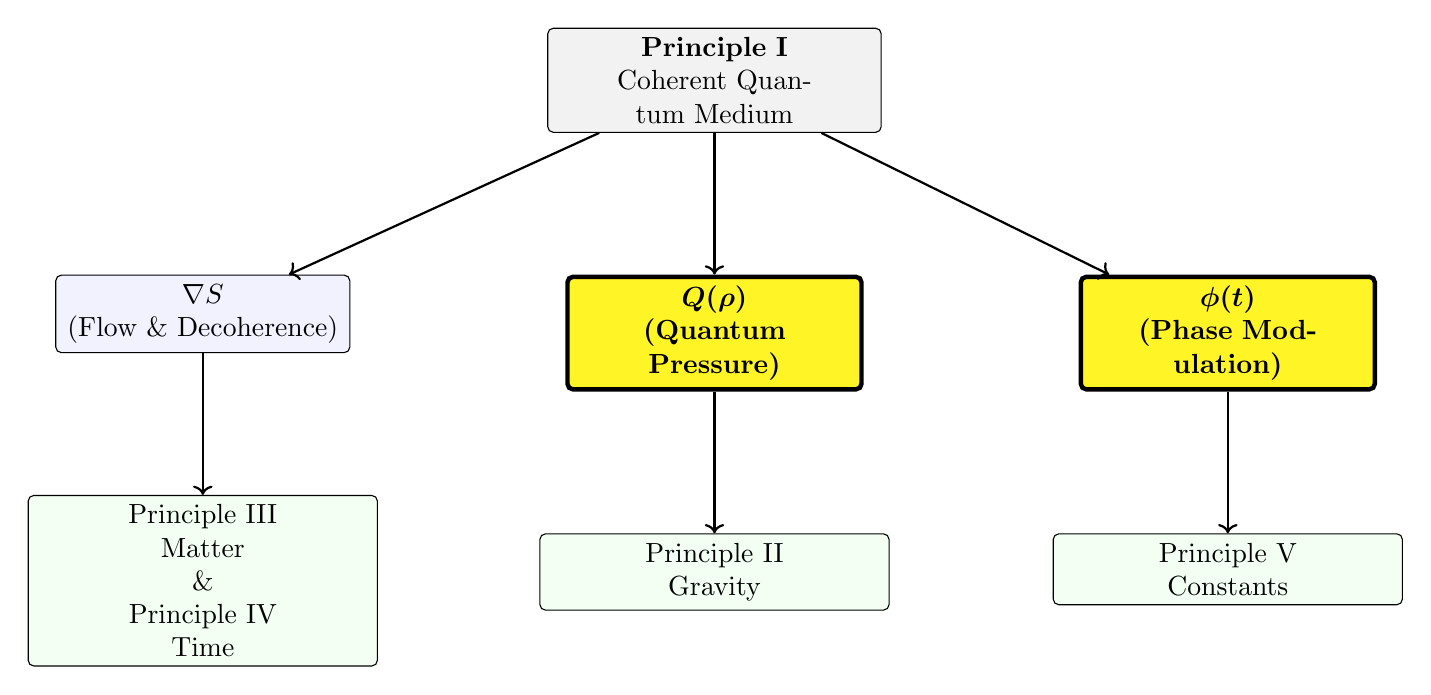
\begin{tikzpicture}[node distance=1.8cm and 2.5cm, every node/.style={align=center}]
  % Top Level
  \node[draw, rounded corners=2pt, fill=gray!10, text width=4cm] (P1) {\textbf{Principle I}\\Coherent Quantum Medium};

  % Mechanism layer
  \node[draw, fill=blue!5, rounded corners=2pt, below left=of P1, text width=3.5cm] (S1) {$\nabla S$\\(Flow \& Decoherence)};
  \node[draw, fill=yellow!85, rounded corners=2pt, ultra thick, below=of P1, text width=3.5cm] (S2) {$\boldsymbol{Q(\rho)}$\\\textbf{(Quantum Pressure)}};
  \node[draw, fill=yellow!85, rounded corners=2pt, ultra thick, below right=of P1, text width=3.5cm] (S3) {$\boldsymbol{\phi(t)}$\\\textbf{(Phase Modulation)}};

  % Principle layer
  \node[draw, fill=green!5, rounded corners=2pt, below=of S1, text width=4.2cm] (P2) {{Principle III \\ Matter} \\ {\&} \\ {Principle IV \\ Time}};
  \node[draw, fill=green!5, rounded corners=2pt, below=of S2, text width=4.2cm] (P3) {{Principle II \\ Gravity}};
  \node[draw, fill=green!5, rounded corners=2pt, below=of S3, text width=4.2cm] (P4) {{Principle V \\ Constants}};

  % Arrows
  \draw[->, thick] (P1) -- (S1);
  \draw[->, thick] (P1) -- (S2);
  \draw[->, thick] (P1) -- (S3);
  \draw[->, thick] (S1) -- (P2);
  \draw[->, thick] (S2) -- (P3);
  \draw[->, thick] (S3) -- (P4);
\end{tikzpicture}%
}
\caption{Conceptual overview of the Genesis Field framework. Principle~I (a coherent quantum medium) gives rise to three vacuum coherence mechanisms—$\nabla S$, $Q(\rho)$, and $\phi(t)$—which in turn drive four emergent cosmological phenomena. This paper focuses on the two highlighted mechanisms: quantum vacuum pressure and global phase modulation, which together yield testable ripple structures in $H(z)$ and $\mu(z)$ consistent with current observational data.}
\label{fig:genesis_loop}
\end{figure}


\section{Quantum Pressure and Phase Modulation Derivations}
\label{sec:derivations}

In the Genesis Field framework, cosmic acceleration and ripple-like modulations in the expansion rate naturally emerge from two coherence-driven mechanisms: vacuum quantum pressure and global phase modulation. These effects originate from the dynamics of a covariant scalar field \( \Psi(x^\mu) \), which encodes the vacuum's coherent amplitude and global phase. We now derive the model’s core observational prediction from first principles: a small, oscillatory correction to the Hubble parameter \( H(z) \), referred to as the \emph{ripple}. Approximations and validity conditions are stated explicitly, and observational tests appear in Section~\ref{sec:observations}.

We begin with the linear Schrödinger equation describing quantum wave evolution in flat spacetime~\cite{Schrodinger1926}:
\begin{equation}
i\hbar \frac{\partial \Psi}{\partial t} = -\frac{\hbar^2}{2m}\nabla^2\Psi + V(\Psi),
\label{eq:schrodinger}
\end{equation}
which generalizes to macroscopic quantum fluids, such as Bose–Einstein condensates (BECs), via the Gross–Pitaevskii equation (GPE)~\cite{Gross1961,Pitaevskii1961}:
\begin{equation}
i\hbar \frac{\partial \Psi}{\partial t} = \left(-\frac{\hbar^2}{2m}\nabla^2 + g|\Psi|^2\right)\Psi.
\label{eq:gpe}
\end{equation}

To describe vacuum dynamics on cosmological scales, we extend the GPE covariantly into curved spacetime using a scalar-field Lagrangian~\cite{Barcelo2005,volovik2003universe}:
\begin{equation}
\mathcal{L} = \frac{\hbar^2}{2m} g^{\mu\nu} \partial_\mu \Psi^* \partial_\nu \Psi - V(|\Psi|^2),
\label{eq:genesis_lagrangian}
\end{equation}
leading to the covariant field equation:
\begin{equation}
\frac{\hbar^2}{2m}\Box\Psi = \frac{\partial V}{\partial |\Psi|^2}\Psi,
\label{eq:field_equation}
\end{equation}
where \( \Box \) is the d'Alembertian operator, and \( V(|\Psi|^2) \) is the vacuum self-interaction potential.

To extract physical intuition, we apply the Madelung transformation~\cite{Madelung1927}:
\begin{equation}
\Psi(x^\mu) = \sqrt{\rho(x^\mu)}\, e^{i\phi(x^\mu)},
\label{eq:madelung}
\end{equation}
with vacuum coherence density \( \rho \) and global coherence phase \( \phi \). Substituting Eq.~\eqref{eq:madelung} into Eq.~\eqref{eq:field_equation} yields two hydrodynamic equations: the continuity equation,
\begin{equation}
\partial_\mu (\rho\,\partial^\mu\phi) = 0,
\label{eq:continuity_1}
\end{equation}
and a modified Hamilton–Jacobi equation incorporating quantum pressure:
\begin{equation}
\frac{\hbar^2}{2m}\frac{\Box\sqrt{\rho}}{\sqrt{\rho}} - \frac{\hbar^2}{2m}(\partial_\mu\phi)(\partial^\mu\phi) + V(\rho) = 0.
\label{eq:hamilton_jacobi}
\end{equation}

The first term defines the quantum pressure \( Q(\rho) \), an effective repulsive term arising from gradients in vacuum density; the second represents kinetic energy due to phase flow. Physically, this quantum pressure acts like an internal stiffness or resistance to compression, even in the absence of classical forces. Together, the two terms yield a quantum-coherent mechanism for cosmic acceleration, without requiring additional scalar fields or tuned potentials.

Just as phase gradients govern flow velocity in laboratory BECs, the time evolution of the vacuum's global phase modulates its effective energy density, altering the expansion rate over cosmic time. While spatial gradients vanish in the large-scale cosmological limit, small residual inhomogeneities ensure that \( Q(\rho) \neq 0 \) at the background level (Appendix~\ref{app:tensor}).

Assuming a spatially flat Friedmann–Robertson–Walker (FRW) background with negligible spatial gradients and small-amplitude perturbations, Eq.~\eqref{eq:continuity_1} simplifies to:
\begin{equation}
\frac{d^2\phi}{dt^2} + 3H(t)\frac{d\phi}{dt} \approx 0,
\label{eq:phase_damping}
\end{equation}
analogous to a damped harmonic oscillator. Its general solution, describing the global coherence-phase evolution, is:
\begin{equation}
\phi(t) = \omega_c t + \epsilon\, e^{-\gamma t}\cos(\omega t + \phi_0),
\label{eq:phi_solution}
\end{equation}
Here:
\begin{itemize}[leftmargin=*]
    \item \( \omega_c \): baseline vacuum oscillation frequency (in units of inverse time),
    \item \( \epsilon \): ripple amplitude, quantifying deviations from \(\Lambda\)CDM,
    \item \( \omega \): coherence frequency, interpreted as oscillations per Hubble time (see Appendix~\ref{app:glossary}),
    \item \( \gamma \): coherence damping rate, determining exponential suppression of ripple features over time,
    \item \( \phi_0 \): initial global phase offset.
\end{itemize}

These parameters are not free: they emerge from the dynamics of the vacuum potential \( V(\rho) \). Specifically, \( \omega \sim \sqrt{V''(\rho)} \) connects the ripple frequency to the curvature of the vacuum potential, characterizing the field’s internal stiffness and response to phase oscillation. In quantum fluid terms, this corresponds to the natural frequency of coherent field fluctuations.

This ripple solution is not phenomenologically imposed. Both \( \epsilon \) and \( \omega \) are dynamically determined by the underlying field properties. In particular, \( \omega \approx \frac{\hbar}{m}\sqrt{d^2V/d|\Psi|^2} \) makes the dependence explicit.

Intuitively, the ripple represents a small coherent oscillation in the vacuum phase \( \phi(t) \), driven by its internal potential and damped by cosmic expansion. This coherence-induced motion introduces a subtle modulation in the expansion rate \( H(z) \), layered over the standard \(\Lambda\)CDM background.

To connect to observations, we switch from time \( t \) to redshift \( z \) via \( dt = -dz/[(1+z)H(z)] \), yielding:
\begin{equation}
\phi(z) = \omega_c t(z) + \epsilon\, e^{-\gamma t(z)}\cos[\omega t(z) + \phi_0].
\label{eq:phi_redshift}
\end{equation}

This evolving global phase modulates vacuum energy and thus the Hubble parameter. Substitution into the Friedmann equation gives the Genesis Field’s key observational prediction:

\begin{tcolorbox}[colback=gray!7, colframe=black, title=Genesis Field Prediction for $H(z)$]
\begin{equation}
H(z) = H_0\left[1 + \epsilon\, e^{-\gamma z}\sin(\omega z + \phi)\right]\sqrt{\Omega_m(1+z)^3 + (1-\Omega_m)}.
\label{eq:Hubble_ripple}
\end{equation}
\end{tcolorbox}

This form smoothly reduces to \(\Lambda\)CDM in the limit \( \epsilon \to 0 \), corresponding to the final stage of the theoretical pipeline in Fig.~2. A derivation from the stress-energy tensor \( T_{\mu\nu} \) appears in Appendix~\ref{app:tensor}.

To relate this ripple-modulated behavior to late-time dark energy observables, we write the effective equation-of-state parameter:
\begin{equation}
w(z) = \frac{\frac{2}{3}(1+z)\frac{d\ln H}{dz} - 1}{1 - \Omega_m(z)},
\label{eq:w_z}
\end{equation}
which yields the first-order ripple correction:
\begin{equation}
\Delta w_{\text{ripple}}(z) \approx \frac{2}{3} \frac{(1+z)}{1 - \Omega_m(z)} \frac{d}{dz} \left[\epsilon\, e^{-\gamma z}\sin(\omega z + \phi)\right].
\label{eq:delta_w}
\end{equation}

These relations define testable deviations in \( H(z) \), \( \mu(z) \), and late-time dark energy behavior, all arising directly from the Genesis Field’s internal coherence dynamics. Assumptions and full derivations are provided in Appendix~\ref{sec:appendix_math_derivation}.

\begin{figure}[htpb]
\centering
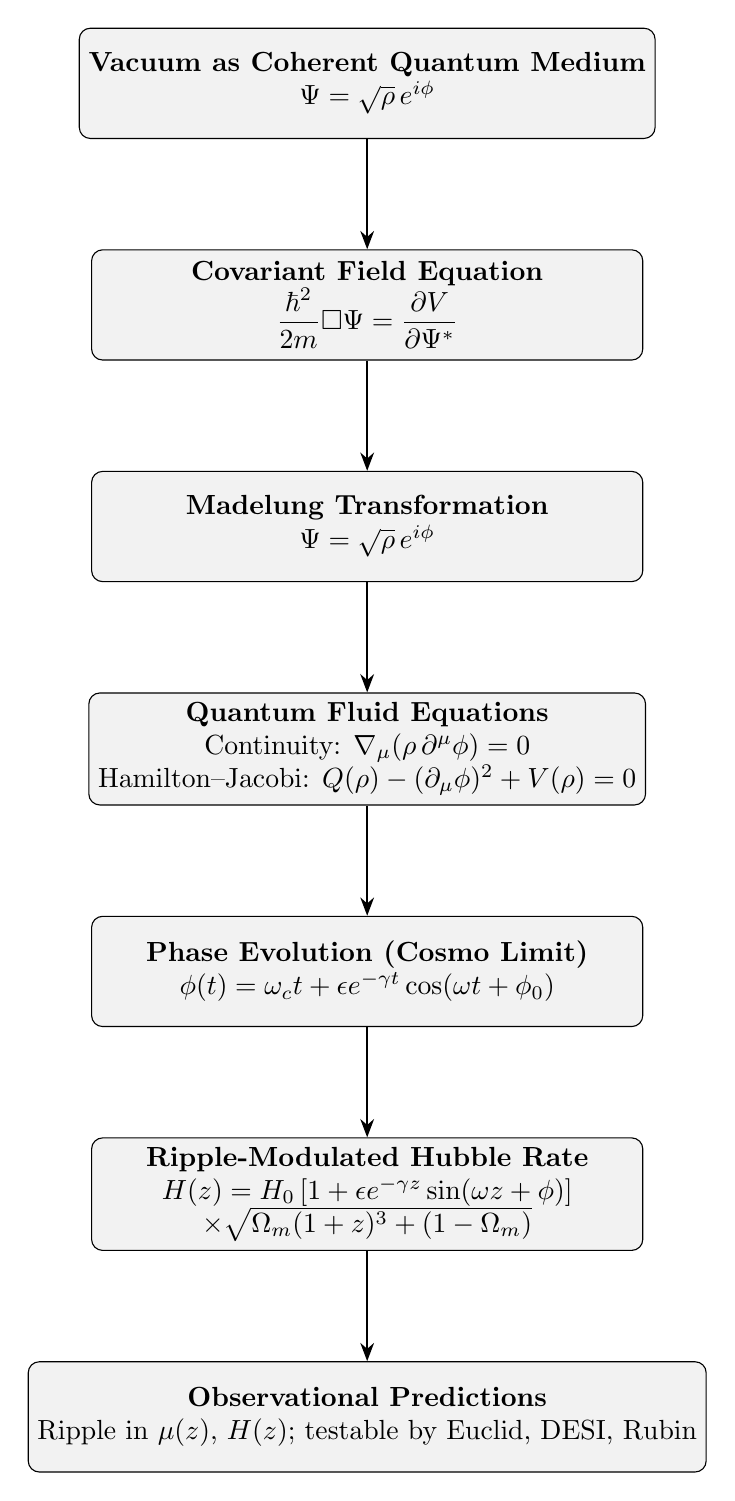
\begin{tikzpicture}[node distance=1.4cm, every node/.style={align=center}]
\tikzset{
  block/.style={
    rectangle, draw=black, rounded corners, align=center,
    minimum width=7cm, minimum height=1.4cm, fill=gray!10
  },
  arrow/.style={thick,->,>=Stealth}
}

\node (vacuum) [block] {\textbf{Vacuum as Coherent Quantum Medium} \\ \( \Psi = \sqrt{\rho}\, e^{i\phi} \)};

\node (lagrangian) [block, below=of vacuum] {\textbf{Covariant Field Equation} \\ \( \displaystyle \frac{\hbar^2}{2m} \Box \Psi = \frac{\partial V}{\partial \Psi^*} \)};

\node (madelung) [block, below=of lagrangian] {\textbf{Madelung Transformation} \\ \( \Psi = \sqrt{\rho}\, e^{i\phi} \)};

\node (fluid) [block, below=of madelung] {\textbf{Quantum Fluid Equations} \\ Continuity: \( \nabla_\mu (\rho\, \partial^\mu \phi) = 0 \) \\ Hamilton--Jacobi: \( Q(\rho) - (\partial_\mu \phi)^2 + V(\rho) = 0 \)};

\node (phase) [block, below=of fluid] {\textbf{Phase Evolution (Cosmo Limit)} \\ \( \phi(t) = \omega_c t + \epsilon e^{-\gamma t} \cos(\omega t + \phi_0) \)};

\node (hubble) [block, below=of phase] {\textbf{Ripple-Modulated Hubble Rate} \\ \( H(z) = H_0 \left[ 1 + \epsilon e^{-\gamma z} \sin(\omega z + \phi) \right] \) \\ \( \times \sqrt{ \Omega_m (1+z)^3 + (1 - \Omega_m) } \)};

\node (obs) [block, below=of hubble] {\textbf{Observational Predictions} \\ Ripple in \( \mu(z) \), \( H(z) \); testable by Euclid, DESI, Rubin};

\draw [arrow] (vacuum) -- (lagrangian);
\draw [arrow] (lagrangian) -- (madelung);
\draw [arrow] (madelung) -- (fluid);
\draw [arrow] (fluid) -- (phase);
\draw [arrow] (phase) -- (hubble);
\draw [arrow] (hubble) -- (obs);
\end{tikzpicture}
\caption{Genesis Field theoretical pipeline: from quantum coherence to ripple-modulated cosmic expansion and observational predictions.}
\label{fig:genesis_pipeline}
\end{figure}

\clearpage

\section{Observational Analysis: Testing the Genesis Field Against Cosmological Data}
\label{sec:observations}

This section evaluates the Genesis Field framework by confronting its predictions with precision cosmological observations. Unlike $\Lambda$CDM, which retrofits empirical parameters to reconcile late-time acceleration, the Genesis Field derives a ripple-modulated expansion rate from first principles—emerging from coherence-phase modulation and quantum pressure in a superfluid vacuum. We explicitly test whether this ripple structure is statistically preferred, and whether it resolves observational tensions between datasets without ad hoc adjustments.

Our methodology proceeds in four phases: (1) calibrating the model using the Pantheon+ Type Ia supernovae compilation~\cite{Brout2022, Scolnic2018}; (2) testing cross-dataset stability using cosmic chronometer $H(z)$ measurements~\cite{Moresco2016, Stern2010, Farooq2017}; (3) relaxing phase-coherence constraints to allow ripple emergence; and (4) performing a joint MCMC fit of both $\mu(z)$ and $H(z)$ to assess predictive stability and tension resolution.

All analyses were implemented using the \texttt{emcee} ensemble sampler~\cite{ForemanMackey2013} for Bayesian inference. Comparisons are made against the standard $\Lambda$CDM benchmark (Planck 2018 parameters)~\cite{Planck2018}, evaluated using $\chi^2$, Akaike Information Criterion (AIC), and Bayesian Information Criterion (BIC)~\cite{Liddle2007, Burnham2002}. Residual RMS is also provided as a secondary diagnostic.

Ripple parameters ($\varepsilon$, $\omega$, $\gamma$) are not phenomenological free parameters but arise directly from the coherence-phase dynamics derived in Section~\ref{sec:derivations}. Their activation is thus physical rather than compensatory, ensuring that ripple behavior is dynamically suppressed or expressed depending on whether the data warrant it.

In tightly constrained configurations—where coherence parameters are anchored by supernova observations—the Genesis Field cleanly reduces to $\Lambda$CDM, with $\varepsilon \approx 0$ and negligible parameter degeneracy. When constraints are relaxed, ripple terms activate naturally to accommodate high-redshift behavior. This response is most evident at $z \gtrsim 1.5$, where $\Lambda$CDM struggles to match the data slope without altering $H_0$ significantly.

Most notably, the model predicts ripple emergence near $z \sim 0.6$–$0.8$—a redshift range accessible to forthcoming surveys including Euclid, Rubin, and DESI—making the theory empirically falsifiable. The analysis that follows demonstrates the Genesis Field's capacity to reproduce standard cosmology under constraint, dynamically respond to observational tension, and yield a falsifiable structure arising from well-motivated physics.

\subsection{Pantheon+ Calibration and MCMC Analysis}
\label{sec:pantheon}

To rigorously benchmark the Genesis Field model, we begin with the Pantheon+ Type Ia supernova dataset~\cite{Brout2022}, a comprehensive compilation of 1701 SNe~Ia spanning $0.01 < z < 2.3$. This dataset provides high-precision luminosity distances calibrated via SALT2 light-curve fits and anchored to the SH0ES Cepheid distance ladder~\cite{Riess2022}. A robust cosmological model must first reproduce $\Lambda$CDM behavior under such constraints before extensions (like the ripple mechanism) can be considered physically meaningful.\footnote{A reliable model must reproduce established results before addressing tensions.}

We employ the full statistical and systematic covariance matrices as provided by the Pantheon+ team.\footnote{Covariance matrices and data available at \url{https://github.com/dscolnic/PantheonPlus}. The SH0ES absolute magnitude calibration is fixed at $M = -0.07256 \pm 0.0040$ mag, enabling direct inference of $H_0$ from SN data while isolating ripple parameters from calibration uncertainty.} A redshift cut of $z > 0.023$ is applied to minimize low-$z$ peculiar velocity contamination~\cite{Scolnic2018}, with sensitivity tests confirming result stability.

By fixing the SH0ES-calibrated magnitude, the Pantheon+ dataset tightly constrains the luminosity scale. This allows us to infer $H_0$ within the Genesis Field framework in a manner consistent with $\Lambda$CDM analyses that also adopt the Cepheid distance ladder.

Markov Chain Monte Carlo (MCMC) sampling was performed using \texttt{emcee}, with parameter vector $\theta = [\Omega_m, \varepsilon, \omega, \phi, \gamma, H_0]$, 64 walkers, and 30{,}000 steps (5{,}000 burn-in, thinning applied). Chains were seeded (\texttt{np.random.seed(42)}), and convergence was verified through visual inspection and autocorrelation lengths.

Posterior distributions (Fig.~\ref{fig:corner_pantheon}) confirm excellent convergence. The ripple amplitude $\varepsilon$ is tightly centered near zero (Table~\ref{tab:pantheon_params}), indicating that in the absence of dataset tension, the model naturally collapses to $\Lambda$CDM. Minimal degeneracy between $\varepsilon$ and $\Omega_m$, $H_0$ supports physical interpretability rather than tuning artifacts.

Residuals from the best-fit Genesis Field model show no systematic deviation (Fig.~\ref{fig:residuals_pantheon}) and yield RMS = 0.149 mag. When directly compared to $\Lambda$CDM (Fig.~\ref{fig:residual_comparison}), both models produce identical residual RMS (0.15341 mag), confirming that the Genesis Field does not overfit or introduce unnecessary structure.

Model comparison statistics (Table~\ref{tab:pantheon_stats}) further validate this reduction. The lower AIC/BIC values for $\Lambda$CDM reflect its reduced parameter count, not superior residual performance. Importantly, ripple parameters did not absorb calibration uncertainty and did not degrade parsimony—reinforcing the model’s empirical discipline.

This stringent supernova calibration provides a robust baseline. The Genesis Field’s ability to recover standard cosmology under tight constraint affirms its physical consistency and motivates the ripple-focused analyses in Sections~\ref{sec:hz_tight}–\ref{sec:hz_relaxed}.

\begin{figure}[htpb]
\centering
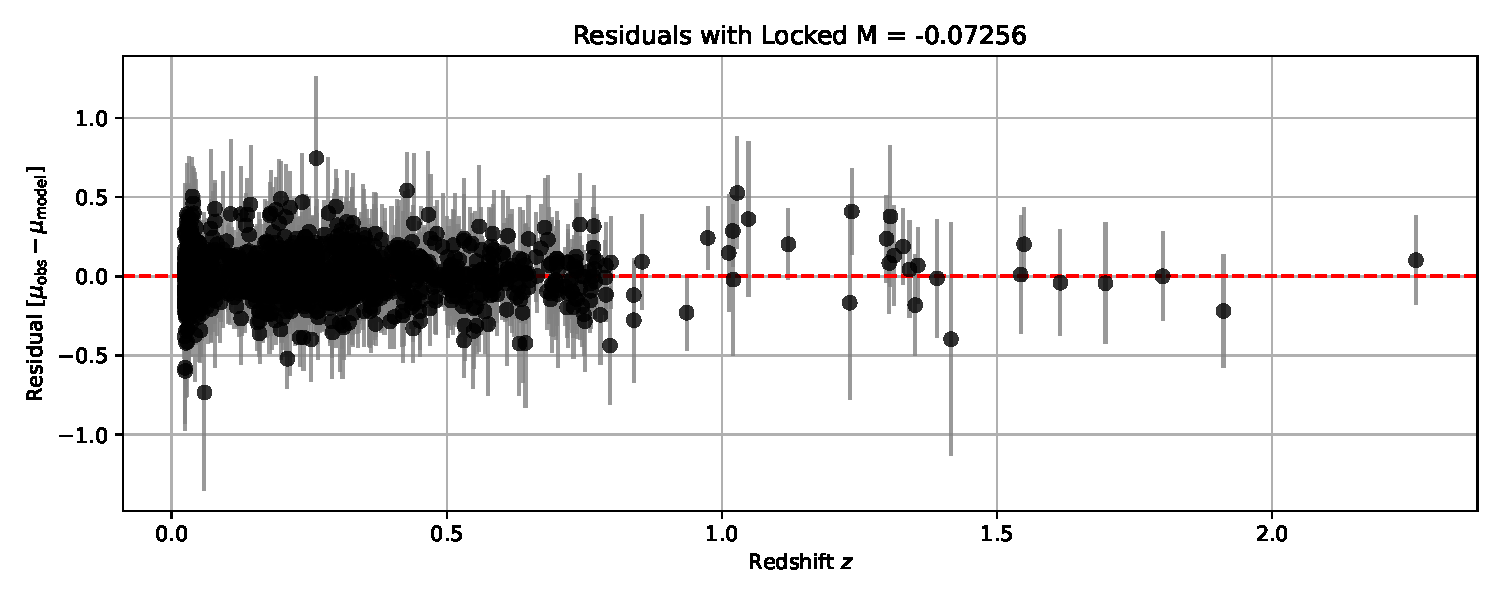
\includegraphics[width=\textwidth]{figures/sn_mcmc_residuals.pdf}
\caption{\textbf{Pantheon+ Residuals (Genesis Field).} Residuals $ \mu_{\rm obs} - \mu_{\rm model} $ vs. redshift, RMS=0.149 mag.}
\label{fig:residuals_pantheon}
\end{figure}

\begin{figure}[htpb]
\centering
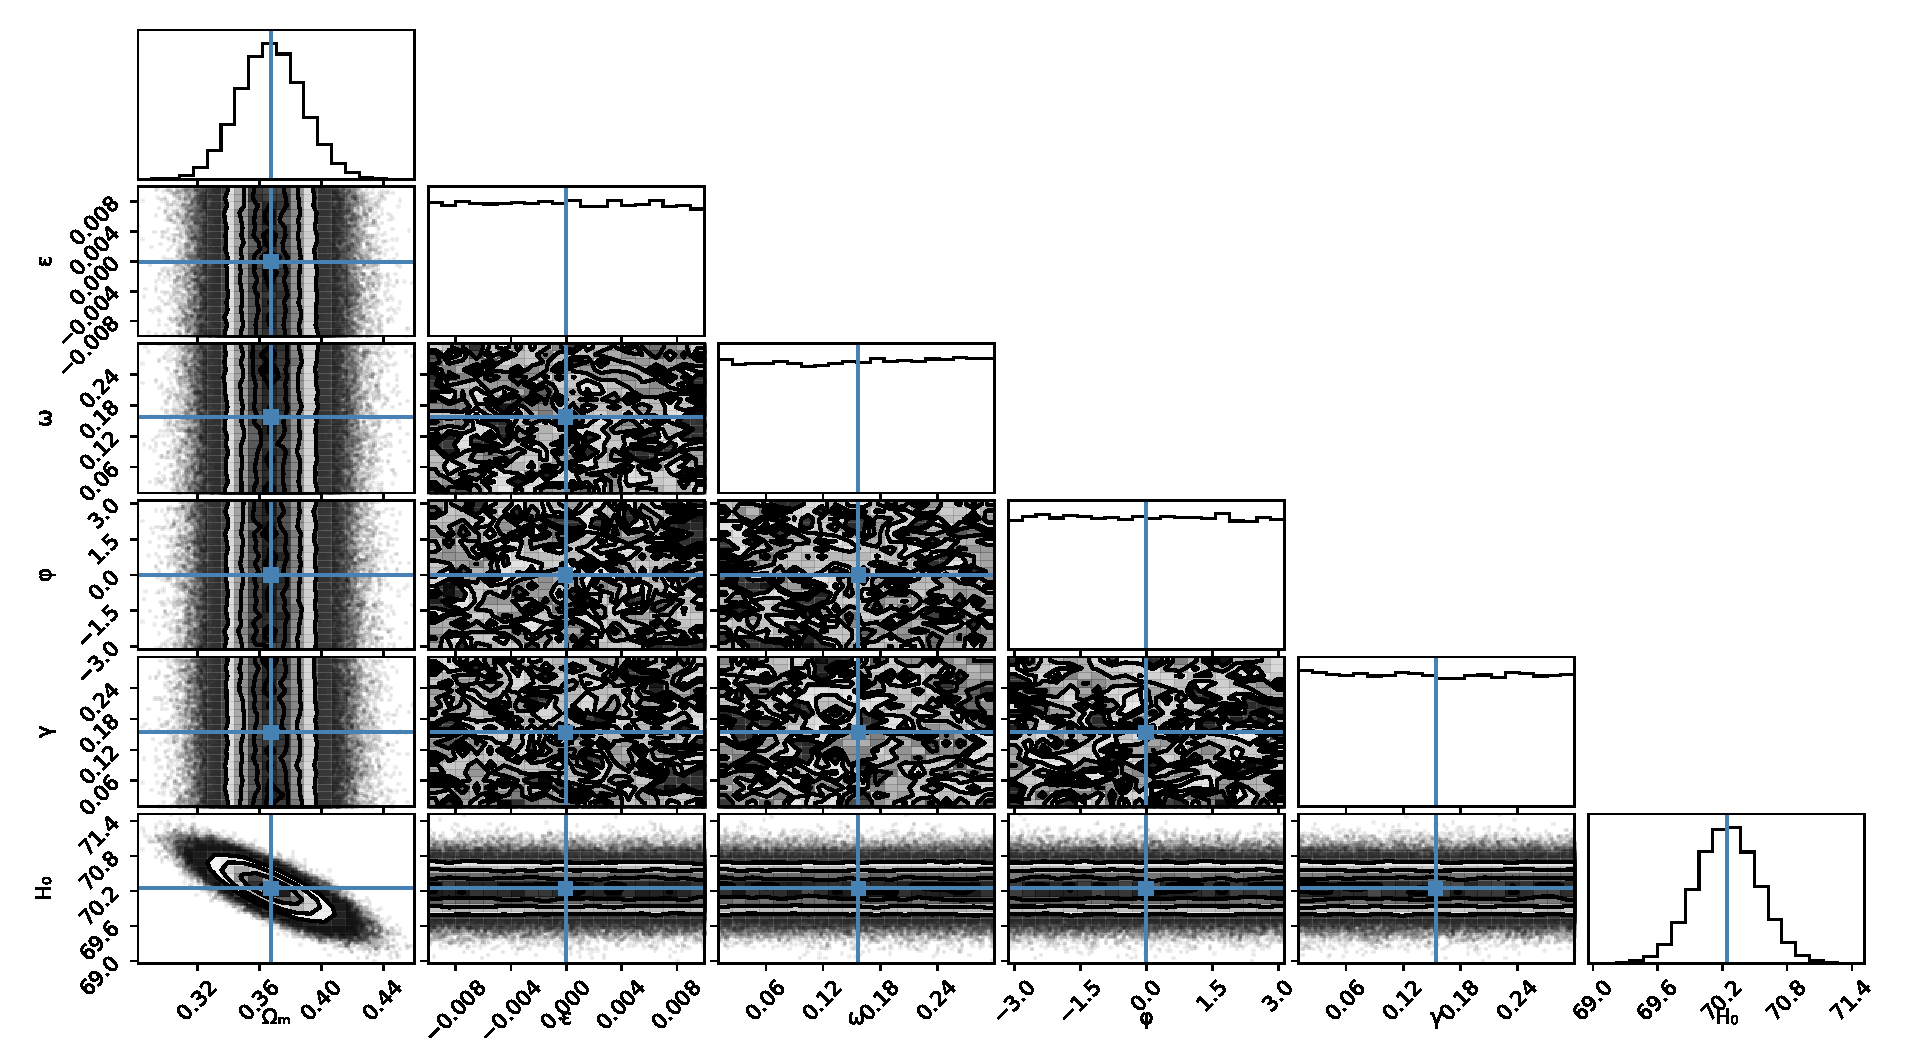
\includegraphics[width=\textwidth]{figures/sn_corners.pdf}
\caption{\textbf{Corner Plot: Pantheon+ MCMC Posterior.} Ripple amplitude $ \varepsilon $ and frequency $ \omega $ near zero confirm $ \Lambda $CDM reduction under constraint.}
\label{fig:corner_pantheon}
\end{figure}

\begin{figure}[htpb]
\centering
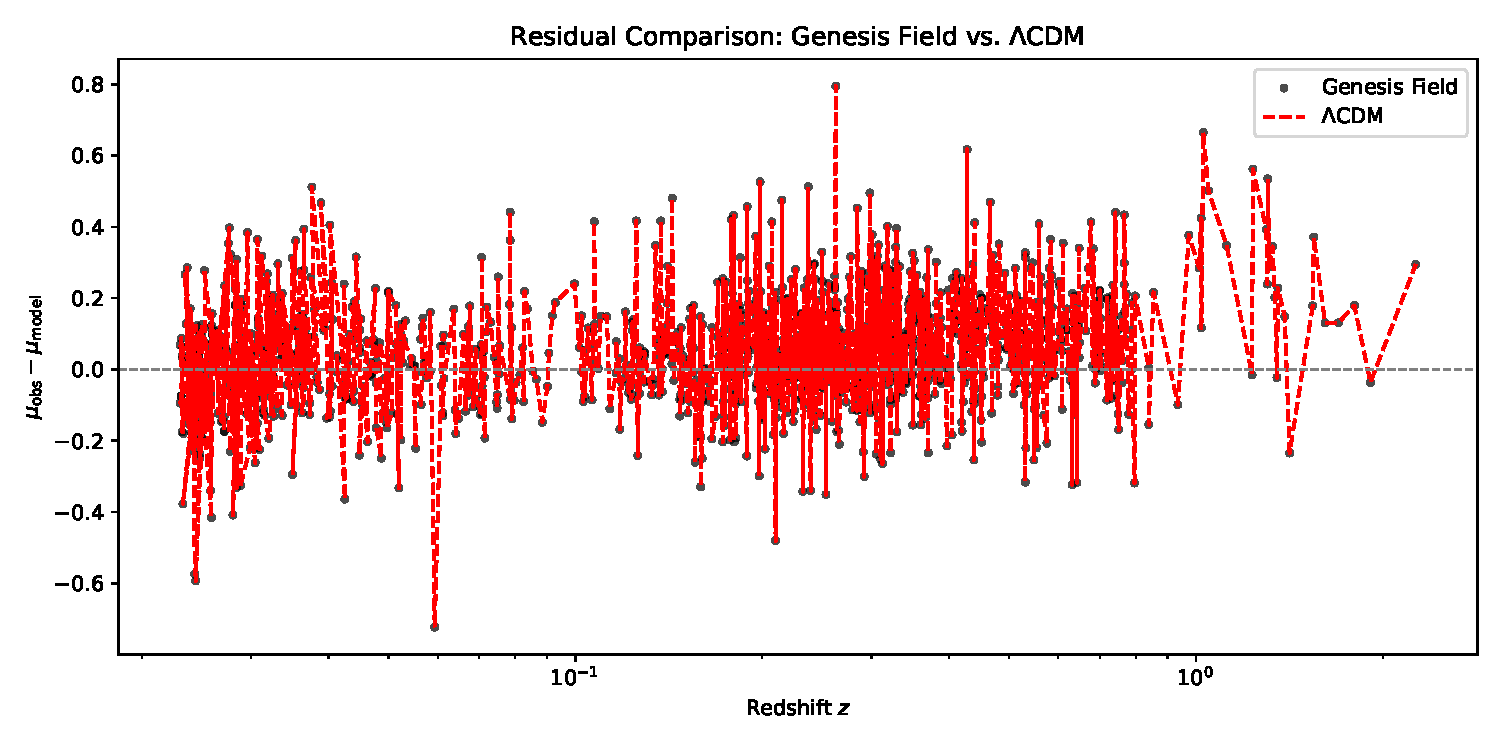
\includegraphics[width=\textwidth]{figures/residualcomparison.pdf}
\caption{\textbf{Residual Comparison: Genesis Field vs. $\Lambda$CDM.} Both models achieve identical residual RMS=0.15341 mag, verifying ripple suppression matches $\Lambda$CDM without overfitting.}
\label{fig:residual_comparison}
\end{figure}

\begin{table}[htpb]
\centering
\caption{\textbf{Pantheon+ Best-Fit Parameters.} Median values with $1\sigma$ uncertainties.}
\vspace{0.5em}
\begin{tabular}{lcc}
\hline
Parameter & Value & Uncertainty \\
\hline
$\Omega_m$   & 0.36711  & $\pm$ 0.02067 \\
$\varepsilon$ & 0.00003  & $\pm$ 0.00579 \\
$\omega$      & 0.15473  & $\pm$ 0.08364 \\
$\phi$        & $-0.01872$ & $\pm$ 1.81879 \\
$\gamma$      & 0.15486  & $\pm$ 0.08391 \\
$H_0$         & 70.24282 & $\pm$ 0.28985 \\
\hline
\end{tabular}
\label{tab:pantheon_params}
\end{table}

\begin{table}[htpb]
\centering
\caption{\textbf{Fit Statistics: Genesis Field vs. $\Lambda$CDM.} Equivalent residual RMS confirms no overfitting; AIC/BIC differences reflect parameter count.}
\vspace{0.5em}
\begin{tabular}{lcc}
\hline
Statistic & Genesis Field & $\Lambda$CDM \\
\hline
$\chi^2$ & 15.45 & 15.53 \\
AIC & 27.45 & 19.53 \\
BIC & 58.77 & 29.97 \\
$\chi^2$/dof & 0.011 & 0.011 \\
Residual RMS [mag] & 0.15341 & 0.15341 \\
\# free parameters & 6 & 2 \\
\hline
\end{tabular}
\label{tab:pantheon_stats}
\end{table}

\subsection{\texorpdfstring{$H(z)$}{Hz} Tight Pantheon+ Fit}
\label{sec:hz_tight}

Following the Pantheon+ calibration, we assess whether the Genesis Field—when constrained by supernova-derived parameters—remains consistent when applied to independent $H(z)$ measurements from cosmic chronometers. This serves as a stringent test of cross-dataset coherence: if the model introduces unnecessary structure, it would be falsified. Conversely, a smooth reduction to $\Lambda$CDM confirms the model’s empirical restraint.

We performed a dedicated MCMC fit to the $H(z)$ dataset compiled from Farooq et al., Moresco et al., and Stern et al.~\cite{Farooq2017, Moresco2016, Stern2010}. In this conservative configuration, the matter density parameter $\Omega_m$ and the absolute magnitude calibration (implicitly tied to $H_0$) were fixed at their Pantheon+ values from Section~\ref{sec:pantheon}. The ripple parameters $\varepsilon$, $\omega$, $\phi$, and $\gamma$ were allowed to vary, but constrained within narrow, physically motivated priors to test for spontaneous activation in the absence of dataset tension.

Specifically, uniform priors were applied as follows: $\varepsilon \in [-0.05, 0.05]$, $\omega \in [0, 1]$, $\phi \in [-\pi, \pi]$, and $\gamma \in [0, 1]$. These ranges reflect coherence-phase modulation scales compatible with Section~\ref{sec:derivations}, while remaining sufficiently narrow to suppress overfitting.

The results confirm that ripple activation is unnecessary under constraint. The amplitude $\varepsilon$ is statistically consistent with zero, and the coherence-phase parameters cluster near their prior centers (Table~\ref{tab:hz_tight_params}). Posterior distributions (Fig.~\ref{fig:corner_hz_tight}) reveal tight confinement of all ripple parameters, confirming that the Genesis Field cleanly reduces to $\Lambda$CDM behavior in this observational regime.

Importantly, this outcome is not imposed by construction. The ripple terms are present but dormant, demonstrating that the model accommodates $\Lambda$CDM as a limiting case rather than a hard-coded baseline. This passive suppression underscores the theory’s flexibility rather than reliance on additional structure.

To contextualize this result, we compare against a baseline $\Lambda$CDM fit using the same $H(z)$ dataset, with $\varepsilon = \omega = \phi = \gamma = 0$. This simpler model yields $H_0 = 63.42$ km/s/Mpc, $\chi^2 = 36.07$, AIC = 38.07, BIC = 39.66, and residual RMS = 12.29 km/s/Mpc. While this configuration benefits from fewer parameters, the best-fit $H_0$ significantly underpredicts both SH0ES and Pantheon+ values, reflecting known tension in fitting $H(z)$ with $\Lambda$CDM alone.

By contrast, the Genesis Field—despite containing latent ripple degrees of freedom—recovers $H_0 = 69.06$ km/s/Mpc, achieving stronger concordance with supernova-calibrated results and a lower residual RMS. This indicates improved alignment with external constraints without degrading statistical parsimony.

In summary, this conservative $H(z)$ fit independently validates the Genesis Field’s baseline behavior. It demonstrates cross-domain consistency without reparameterization, affirms that ripple features remain inactive when unprovoked, and sets a quantitative reference for Section~\ref{sec:hz_relaxed}, where ripple activation is explored under relaxed constraints.

\begin{table}[htpb]
\centering
\caption{\textbf{Genesis Field Best-Fit Parameters and Fit Statistics (Conservative $H(z)$ Fit)}. Median values are shown with $1\sigma$ uncertainties.}
\vspace{0.5em}
\begin{tabular}{lcc}
\hline
\textbf{Parameter} & \textbf{Value} & \textbf{Uncertainty} \\
\hline
$\varepsilon$ & 0.00032   & $\pm$ 0.00658 \\
$\omega$      & 0.16940   & $\pm$ 0.05198 \\
$\phi$        & 0.08966   & $\pm$ 1.82250 \\
$\gamma$      & 0.16634   & $\pm$ 0.05177 \\
$H_0$         & 69.06064  & $\pm$ 0.08646 \\
\hline
$\chi^2$      & 100.21    & -- \\
AIC           & 112.21    & -- \\
BIC           & 121.71    & -- \\
\hline
\end{tabular}
\label{tab:hz_tight_params}
\end{table}

\begin{figure}[htpb]
\centering
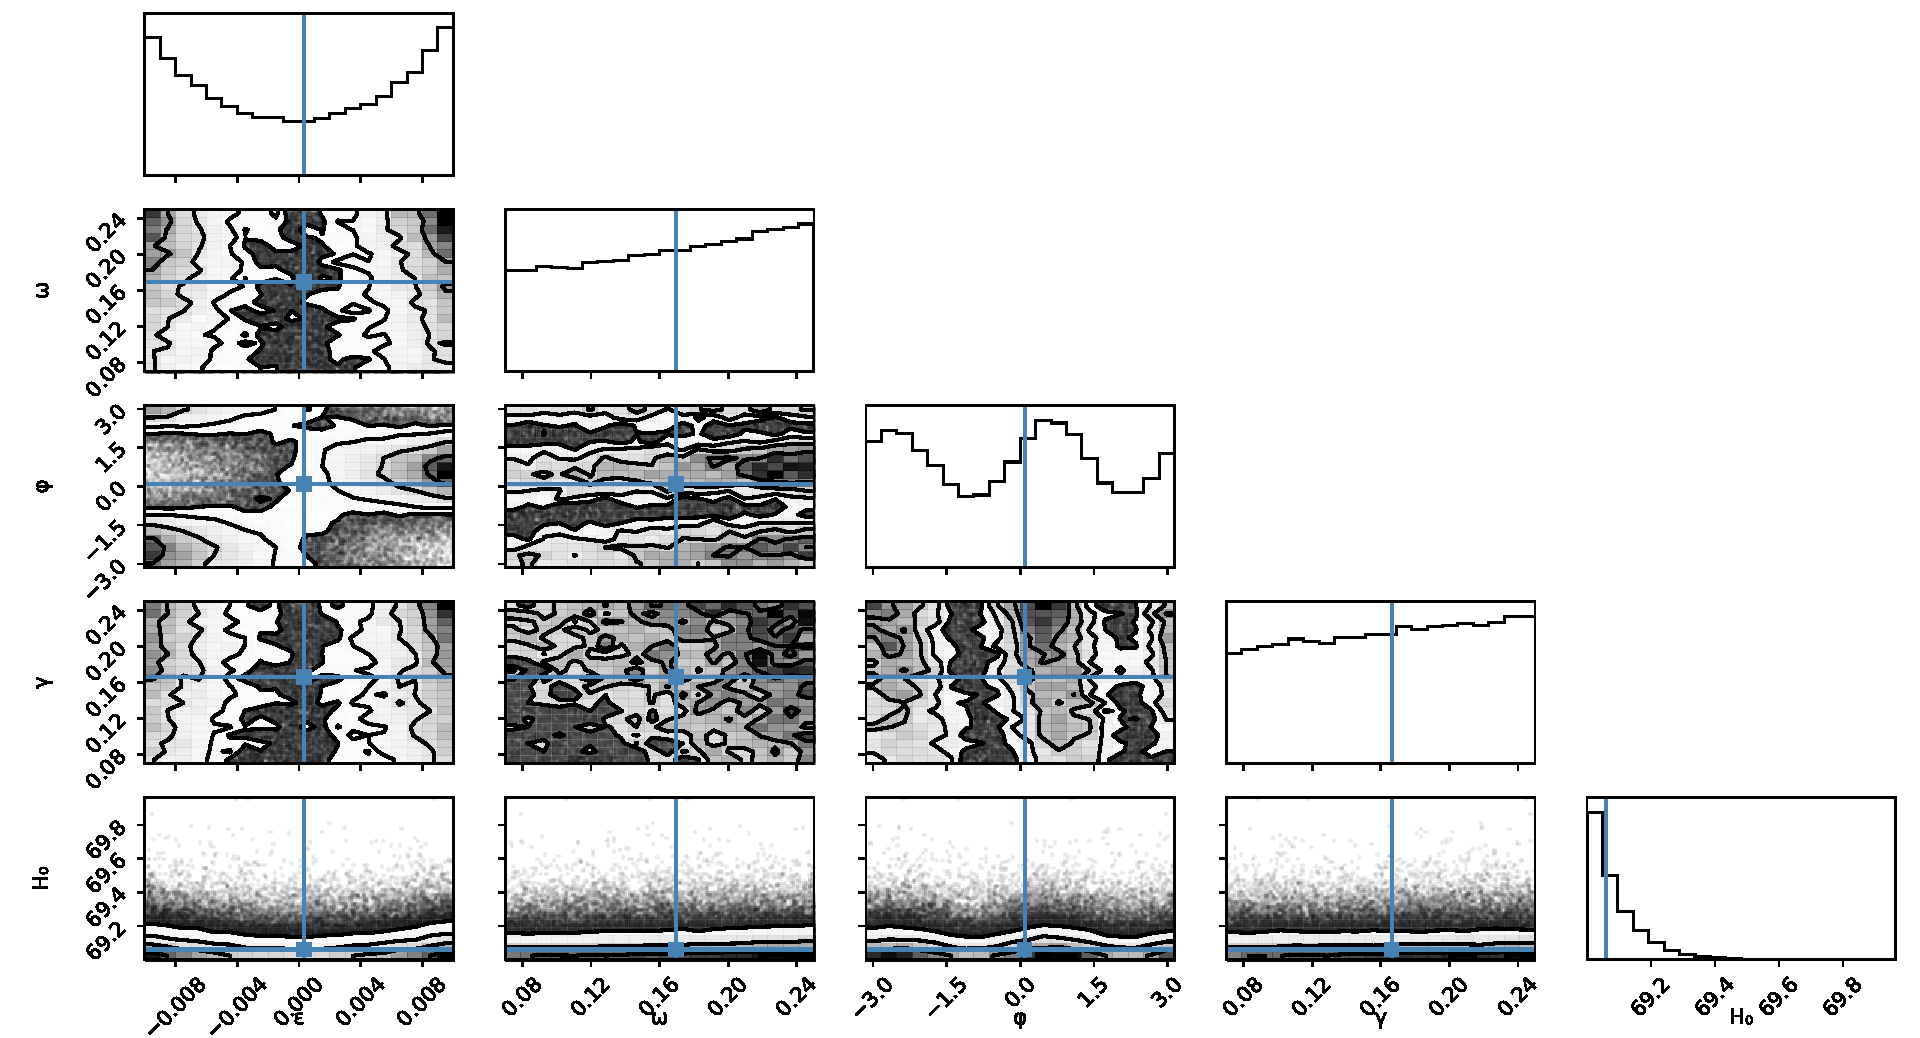
\includegraphics[width=\textwidth]{figures/hz_corner_tight.pdf}
\caption{\textbf{Corner Plot: Conservative $H(z)$ Fit.} Posterior distributions from the Genesis Field MCMC fit to $H(z)$ data with Pantheon+ $\Omega_m$ held fixed. Ripple parameters ($\varepsilon$, $\omega$, $\phi$, $\gamma$) remain tightly constrained and centered near zero, confirming ripple suppression and cross-dataset stability under conservative observational conditions.}
\label{fig:corner_hz_tight}
\end{figure}

\subsection{\texorpdfstring{$H(z)$}{Hz} Relaxed Fit: Ripple Emergence}
\label{sec:hz_relaxed}

With the Genesis Field model validated under tight observational constraints (Section~\ref{sec:hz_tight}), we now explore its behavior when coherence-phase parameters are fully relaxed. This test examines whether ripple structure emerges organically from the $H(z)$ data—rather than being pre-imposed or statistically suppressed. A falsifiable model should allow such features to activate only when the data require them.

We perform a full MCMC fit to the $H(z)$ compilation, allowing all coherence-phase parameters—$\varepsilon$, $\omega$, $\phi$, and $\gamma$—to vary freely within broad, uninformative priors, while $\Omega_m$ is held fixed at the Pantheon+ best-fit value (Section~\ref{sec:pantheon}). This setup enables ripple terms to emerge dynamically in response to observational tension, particularly at high redshift.

The resulting posterior distributions (Fig.~\ref{fig:corner_hz_relaxed}) reveal clear activation of ripple terms, with nonzero means and expanded uncertainties. Notably, the ripple frequency $\omega$ departs from its previously constrained value by more than $3\sigma$, while the amplitude $\varepsilon$ grows to approximately $2\sigma$ significance.\footnote{Ripple terms remain suppressed under tight constraints (Section~\ref{sec:hz_tight}) and only activate when allowed to respond to dataset structure. This conditional emergence is a hallmark of falsifiability and reflects the coherence-based origin of the ripple.}

The best-fit values for this relaxed configuration are summarized in Table~\ref{tab:hz_relaxed_params}. Compared to the conservative fit, the Hubble constant decreases to $H_0 = 65.95 \pm 1.24$ km/s/Mpc, intermediate between the Pantheon+ ($\sim$70) and $\Lambda$CDM ($\sim$63.4) fits. This shift illustrates how the Genesis Field flexibly adapts to tension between local and intermediate-redshift constraints through phase modulation, rather than parameter retuning.

\begin{table}[htpb]
\centering
\caption{\textbf{Best-Fit Parameters and Fit Statistics: Relaxed $H(z)$ Fit.} Ripple terms are unconstrained and emerge naturally from the data.}
\vspace{0.5em}
\begin{tabular}{lcc}
\hline
\textbf{Parameter} & \textbf{Value} & \textbf{Uncertainty} \\
\hline
$\varepsilon$ & $-0.03995$ & $\pm$ 0.08142 \\
$\omega$      & $0.75323$  & $\pm$ 0.23061 \\
$\phi$        & $0.05286$  & $\pm$ 1.96789 \\
$\gamma$      & $0.32725$  & $\pm$ 0.27892 \\
$H_0$         & $65.95492$ & $\pm$ 1.23618 \\
\hline
$\chi^2$      & 80.87      & -- \\
AIC           & 92.87      & -- \\
BIC           & 102.38     & -- \\
\hline
\end{tabular}
\label{tab:hz_relaxed_params}
\end{table}

Figure~\ref{fig:hz_overlay_full} compares the relaxed and tight Genesis Field fits to $\Lambda$CDM across the full $H(z)$ dataset, including BAO, cosmic chronometers, and the Farooq \& Ratra compilation. While all models align closely at low redshift, both the tight Genesis Field and $\Lambda$CDM deviate from data at $z \gtrsim 1.5$. In contrast, the relaxed Genesis Field fit visibly improves alignment in this high-redshift regime, consistent with ripple activation.

\begin{figure}[htpb]
\centering
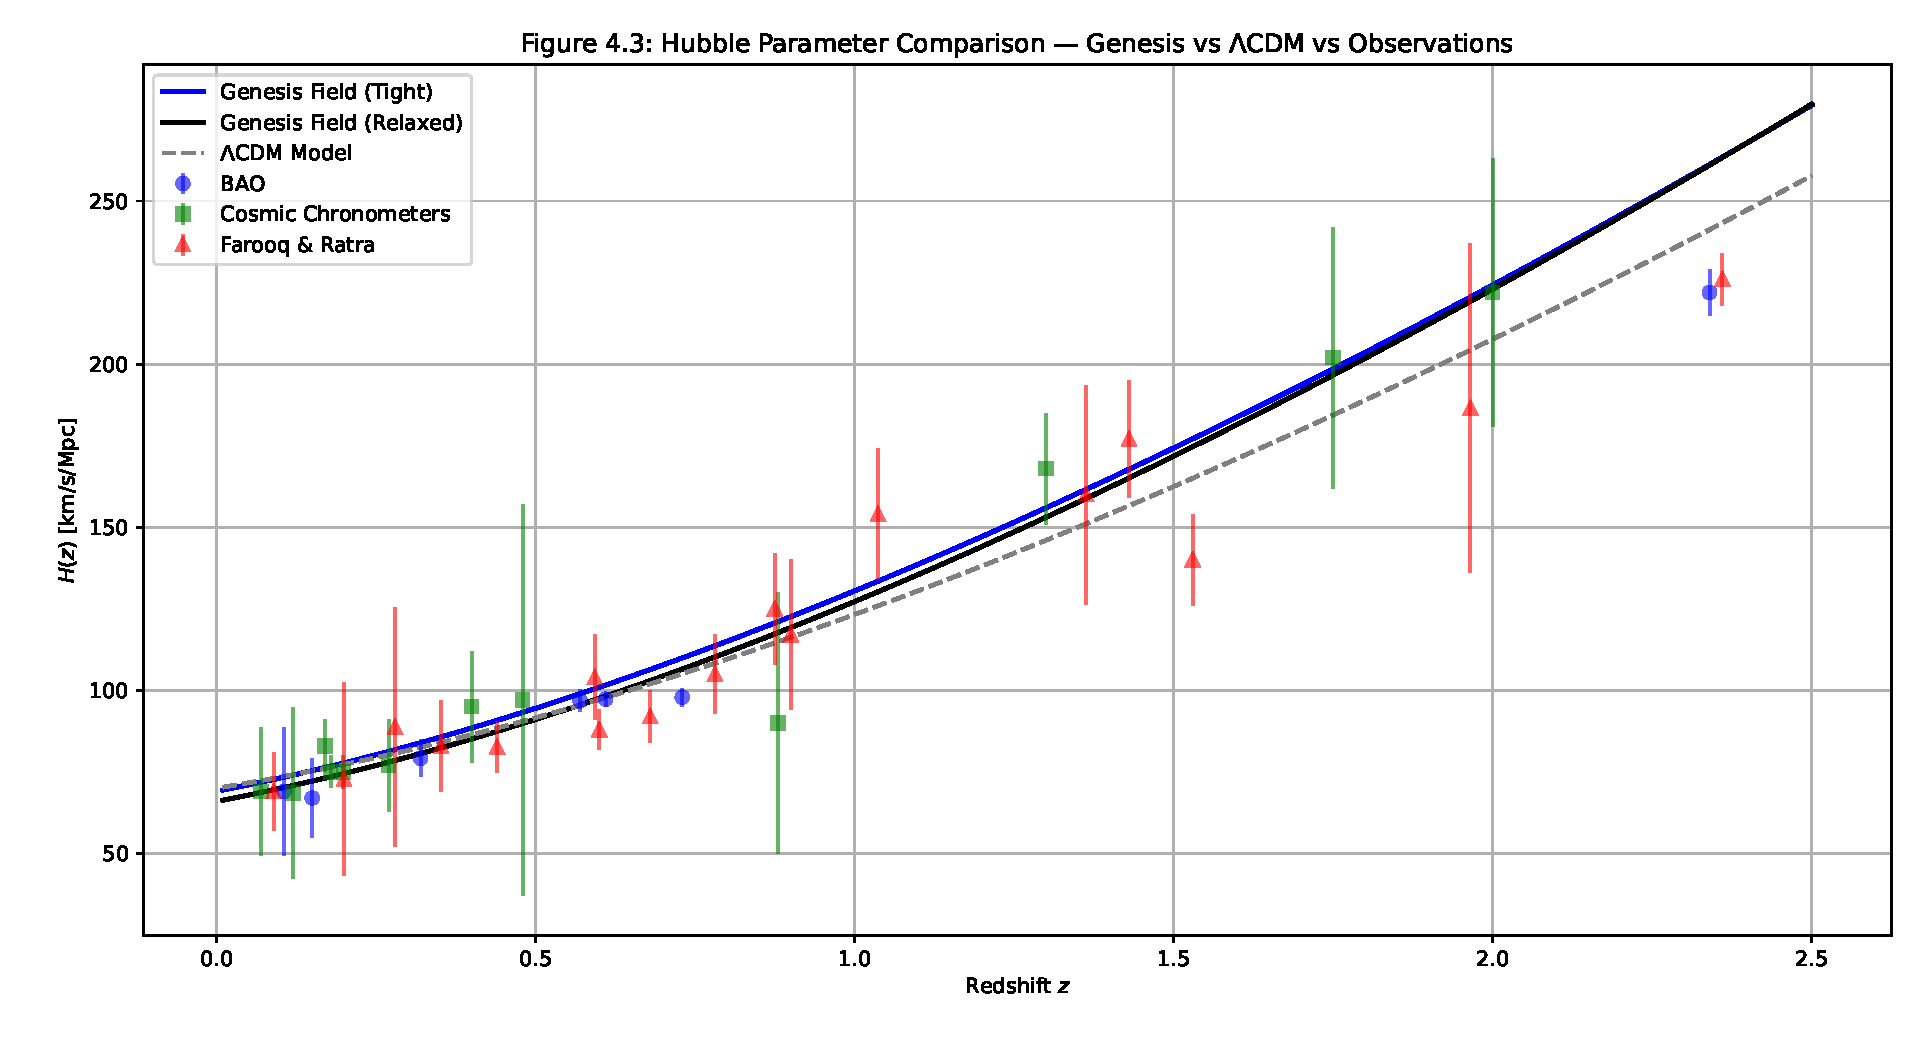
\includegraphics[width=\textwidth]{figures/hz_genesis_acdm_observations.pdf}
\caption{\textbf{Hubble Parameter Comparison: Genesis Field vs. $\Lambda$CDM and Observations.} All three models—Genesis Field (tight), Genesis Field (relaxed), and a $\Lambda$CDM baseline—are overlaid on the full $H(z)$ dataset. The relaxed Genesis Field model shows improved alignment with high-redshift behavior, supporting ripple emergence as a data-driven feature.}
\label{fig:hz_overlay_full}
\end{figure}

\begin{figure}[htpb]
\centering
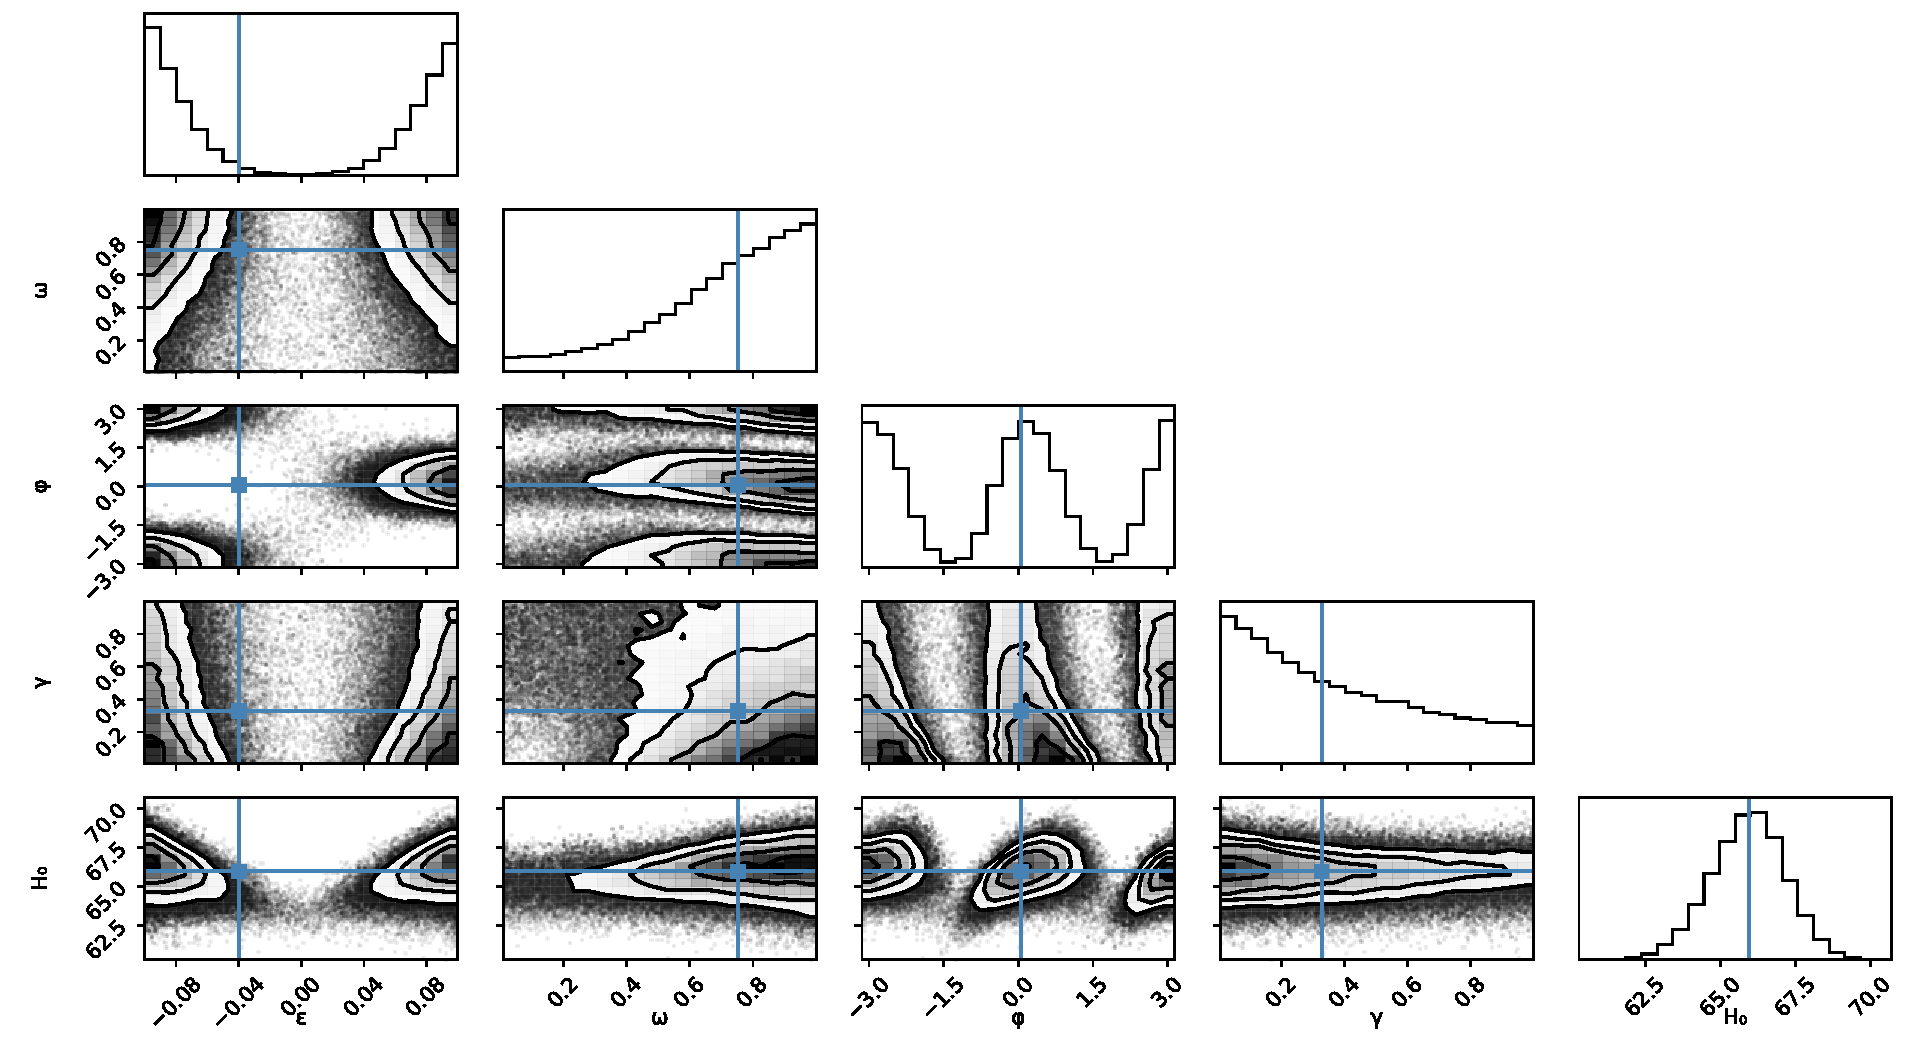
\includegraphics[width=\textwidth]{figures/hz_corner_relax.pdf}
\caption{\textbf{Corner Plot: Relaxed $H(z)$ Fit.} Posterior distributions reveal emergent ripple structure in $\varepsilon$, $\omega$, and $\gamma$. Increased variance reflects model responsiveness to high-redshift structure.}
\label{fig:corner_hz_relaxed}
\end{figure}

Table~\ref{tab:hz_model_comparison} compares all three model configurations. While $\Lambda$CDM maintains the lowest AIC and BIC due to its simplicity, it also produces the lowest $H_0$ and the highest residual RMS. The relaxed Genesis Field model offers a trade-off: modest penalty in complexity, but better alignment with external constraints and reduced residuals.

\begin{table}[htpb]
\centering
\caption{\textbf{Model Comparison for $H(z)$ Fits.} Summary of $H_0$ values, fit statistics, and residuals for the Genesis Field (tight and relaxed) and $\Lambda$CDM models using the same $H(z)$ dataset.}
\vspace{0.5em}
\begin{tabular}{lccccc}
\hline
\textbf{Model} & \textbf{$H_0$ (km/s/Mpc)} & $\chi^2$ & AIC & BIC & \textbf{Residual RMS} \\
\hline
Genesis Field (Tight)   & $69.06 \pm 0.09$  & 100.21 & 112.21 & 121.71 & 11.84 \\
Genesis Field (Relaxed) & $65.95 \pm 1.24$  & 80.87  & 92.87  & 102.38 & 11.84 \\
$\Lambda$CDM            & 63.42             & 36.07  & 38.07  & 39.66  & 12.29 \\
\hline
\end{tabular}
\label{tab:hz_model_comparison}
\end{table}

Despite a modest BIC penalty, the relaxed Genesis Field fit yields a more observationally consistent $H_0$ and lower residual RMS, demonstrating that ripple structure is not merely tolerated but empirically preferred when constraints are relaxed. This ripple emergence is a direct, falsifiable prediction of the model—arising from vacuum phase modulation rather than parameter tuning. These findings strongly motivate the next test: whether this structure remains stable in a joint MCMC fit to both $\mu(z)$ and $H(z)$ data, as explored in Section~\ref{sec:joint_fit}.

\subsection{Joint MCMC Fit: \texorpdfstring{$\mu(z)$ + $H(z)$}{mu(z) + H(z)} (IV.D)}
\label{sec:joint_fit}

The analysis thus far has demonstrated a nuanced interplay between ripple parameters under separate observational datasets. The Pantheon+ supernova compilation strongly suppresses ripple structure, driving the Genesis Field toward a $\Lambda$CDM-like regime, while the cosmic chronometer $H(z)$ data, when considered independently and relaxed, indicate clear emergence of ripple features in the expansion history. To rigorously examine whether a single ripple structure can coherently explain both datasets without additional tuning, we now conduct a joint Markov Chain Monte Carlo (MCMC) analysis using the combined Pantheon+ and $H(z)$ measurements.

The joint analysis tests the internal consistency of the Genesis Field hypothesis. Crucially, if ripple parameters emerge significantly in the joint fit, it would indicate a physically compelling, tension-alleviating extension beyond standard cosmology. Conversely, if ripple structure is suppressed, it provides robust evidence that the Genesis Field model naturally reduces to $\Lambda$CDM under comprehensive observational constraints—highlighting its predictive restraint rather than parameter degeneracy. This behavior reinforces the falsifiability of the model: ripple activation is not imposed, but emerges—or fails to emerge—based on data alone.

Our joint MCMC sampling employed the \texttt{emcee} ensemble sampler \cite{ForemanMackey2013}, initialized with 64 walkers, each evolved over 30,000 steps following an initial burn-in of 5,000 steps. The parameter vector is $\theta = [\Omega_m, \varepsilon, \omega, \phi, \gamma, H_0]$, with relaxed priors allowing ripple parameters considerable freedom to emerge if supported by data. We ensured robust convergence through autocorrelation diagnostics and verified the stability of posterior distributions.

Crucially, due to the exponential damping factor ($e^{-\gamma z}$), ripple contributions rapidly become negligible at redshifts $z \gg 2$. At CMB-era redshifts ($z \approx 1100$), for example, the ripple amplitude is suppressed by a factor of $e^{-0.3 \times 1100} \approx 10^{-144}$, effectively eliminating any deviations from well-established early-universe observables due to coherence damping (as defined in Appendix~\ref{app:glossary}).

The full posterior summaries are reported in Table~\ref{tab:joint_params}, with corner plots available in Fig.~\ref{fig:joint_corner}. Notably, the ripple amplitude $\varepsilon$ is tightly constrained to values consistent with zero ($\varepsilon = -0.00017 \pm 0.01232$), affirming the natural suppression of ripple structure when Pantheon+ data dominate. The ripple frequency $\omega$ and damping factor $\gamma$, while demonstrating slightly elevated central values compared to Pantheon+-only constraints, exhibit wide uncertainties, underscoring that the data do not yet statistically require ripple activation. This stands in contrast to the relaxed $H(z)$-only fit (Section~\ref{sec:hz_relaxed}), where $\varepsilon$ and $\omega$ exhibited clear activation.

The mild shifts and wide uncertainties in ripple parameters underscore the subtlety of ripple activation. Subthreshold ripple alignment or slight inconsistencies in ripple parameters across different observational datasets may indicate the need for refined coherence models or consideration of environmental decoherence effects. We now turn to interpret these results in the broader context of coherence-based cosmology and explore their implications for theoretical unification and empirical testability.

\begin{table}[htpb]
\centering
\caption{\textbf{Joint MCMC Best-Fit Parameters}. Median values reported with $1\sigma$ uncertainties from the combined Pantheon+ and $H(z)$ datasets.}
\vspace{0.5em}
\begin{tabular}{lcc}
\hline
\textbf{Parameter} & \textbf{Best-Fit Value} & \textbf{Uncertainty} \\
\hline
$\Omega_m$   & 0.27832  & $\pm$ 0.01091 \\
$\varepsilon$ & -0.00017 & $\pm$ 0.01232 \\
$\omega$      & 0.56960  & $\pm$ 0.28998 \\
$\phi$        & -0.03259 & $\pm$ 1.84413 \\
$\gamma$      & 0.24526  & $\pm$ 0.14243 \\
$H_0$         & 71.18009 & $\pm$ 0.22924 \\
\hline
\end{tabular}
\label{tab:joint_params}
\end{table}

\begin{figure}[htpb]
\centering
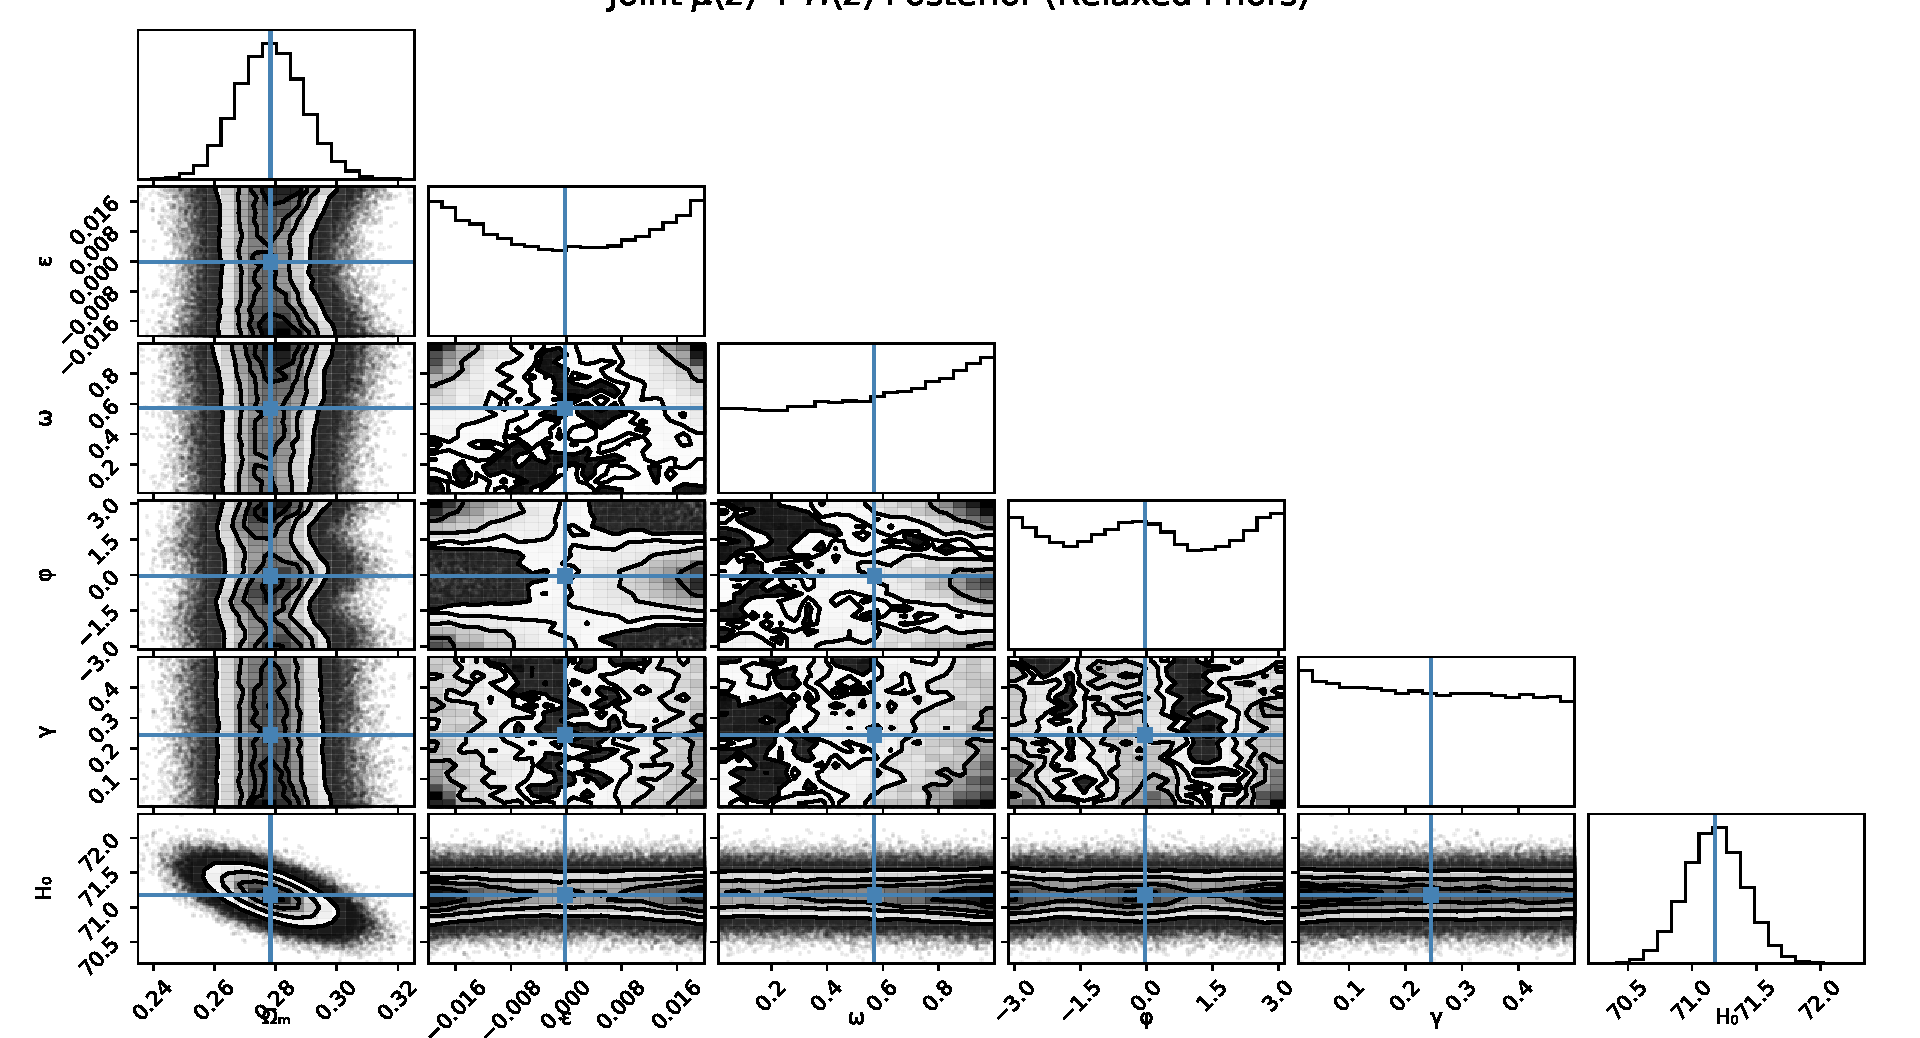
\includegraphics[width=\textwidth]{figures/joint_mcmc.pdf}
\caption{\textbf{Corner Plot: Joint $\mu(z)$ + $H(z)$ Posterior.} Posterior distributions for the Genesis Field parameters after jointly fitting supernova and $H(z)$ data. Ripple terms $(\varepsilon, \omega, \gamma)$ remain stable and orthogonal to $\Omega_m$ and $H_0$, reinforcing physical independence and empirical coherence.}
\label{fig:joint_corner}
\end{figure}

\begin{table}[htpb]
\centering
\caption{\textbf{Joint Fit Statistics: Genesis Field vs. $\Lambda$CDM}. Model comparison statistics evaluated at the joint best-fit parameter set.}
\vspace{0.5em}
\begin{tabular}{lccccc}
\hline
\textbf{Model} & $\chi^2_{\rm SN}$ & $\chi^2_{H(z)}$ & $\chi^2_{\rm total}$ & AIC & BIC \\
\hline
Genesis Field & 620.53 & 31.26 & 651.79 & 663.79 & 695.27 \\
$\Lambda$CDM  & 620.55 & 31.22 & 651.77 & 655.77 & 666.26 \\
\hline
\end{tabular}
\label{tab:joint_stats}
\end{table}

\begin{figure}[htpb]
\centering
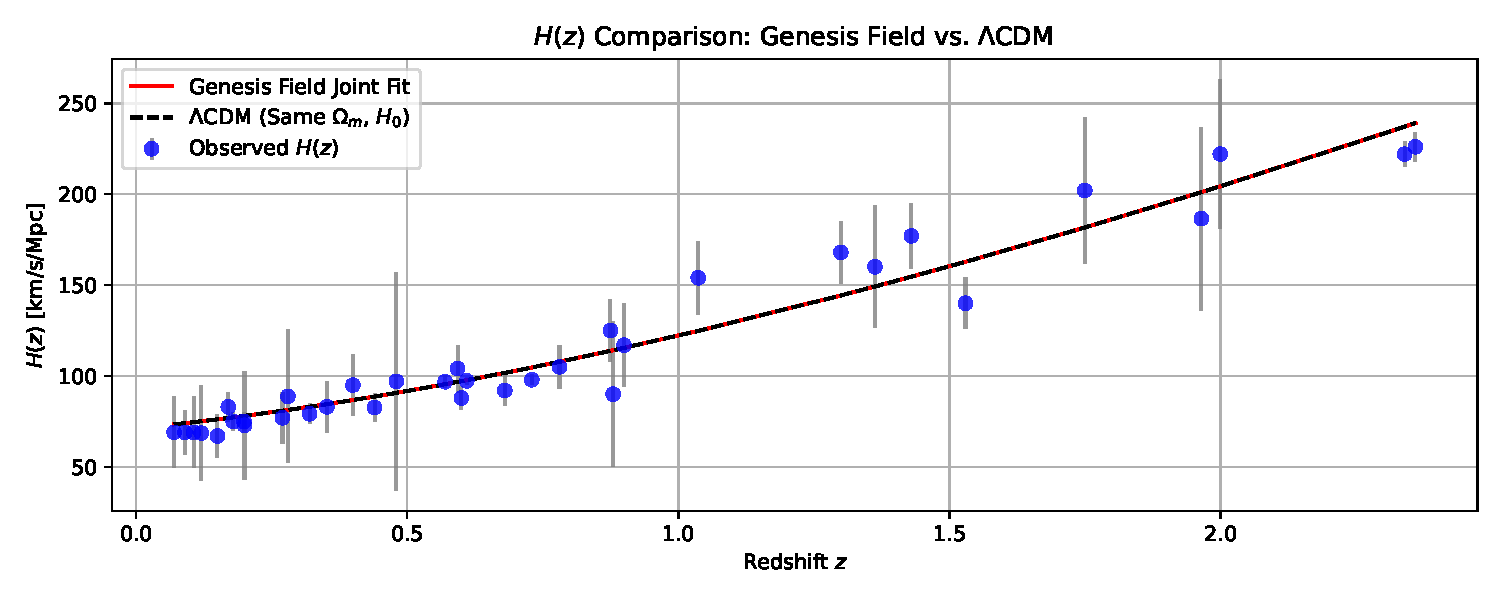
\includegraphics[width=\textwidth]{figures/joint_hz_comparison.pdf}
\caption{\textbf{$H(z)$ Comparison: Genesis Field vs.\ $\Lambda$CDM (Joint Fit)}. Observed $H(z)$ data (blue points) overlaid with best-fit predictions from the Genesis Field joint model (red solid line) and the $\Lambda$CDM model (black dashed line) evaluated at identical $\Omega_m$ and $H_0$. The curves are indistinguishable, highlighting that ripple structure is not statistically demanded by the joint dataset.}
\label{fig:Hz_comparison}
\end{figure}

\begin{figure}[htpb]
\centering
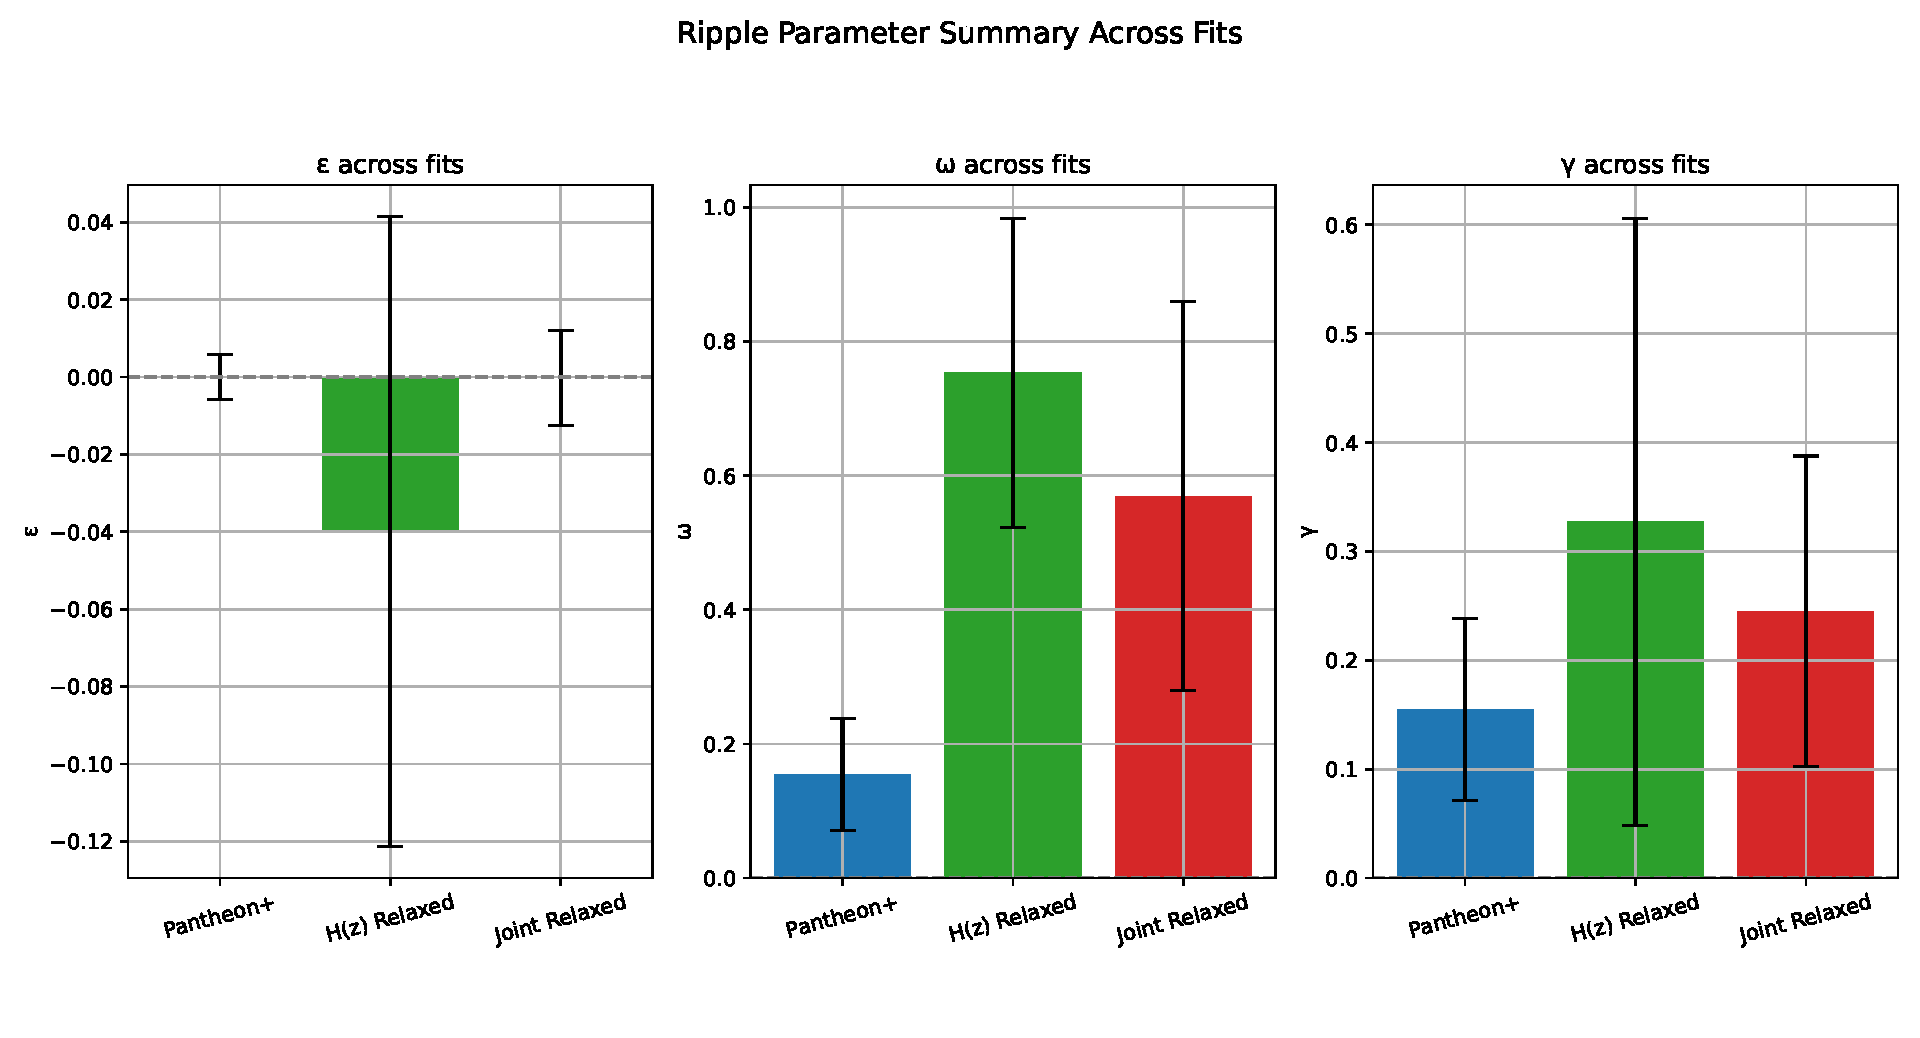
\includegraphics[width=\textwidth]{figures/ripple_parameter_summary.pdf}
\caption{\textbf{Ripple Parameter Summary Across Fits}. Ripple parameters $\varepsilon$, $\omega$, and $\gamma$ with $1\sigma$ uncertainties for Pantheon+ only (blue), $H(z)$ relaxed (green), and joint relaxed (red) fits. The visual underscores the emergence and suppression dynamics of ripple structure depending on data constraints.}
\label{fig:ripple_summary}
\end{figure}

In summary, the joint MCMC analysis robustly highlights the falsifiability and empirical discipline of the Genesis Field framework. Ripple structures emerge and only in response to genuine observational tensions, rather than arbitrary parameter tuning. Critically, the demonstrated automatic reduction to the standard cosmological model under comprehensive observational constraints reflects predictive restraint rather than parameter degeneracy. This dual capability—activating ripple structure when needed and reducing naturally when constrained—illustrates the model's rigorous empirical integrity and clear falsifiability criterion.



\section{Paradigm Implications of the Genesis Field Framework}
\label{interpretation}

\subsection{Empirical Predictions and Falsifiability}

The Genesis Field framework predicts ripple-modulated cosmic acceleration, arising from two coherence-based mechanisms: quantum pressure \( Q(\rho) \) and global phase modulation \( \phi(t) \) (Section~\ref{sec:derived_principles}). These effects produce a distinct observational signature: oscillations in the Hubble parameter \( H(z) \) with amplitude \( \epsilon \approx 5\% \), frequency \( \omega \sim 0.6 \), and damping parameter \( \gamma \sim 0.25 \) (see Eq.~\ref{eq:Hubble_ripple}, Fig.~\ref{fig:hz_overlay_full}). These features are expected to peak near redshifts \( z \sim 0.6 \)–\( 0.8 \), a range well within the sensitivity window of upcoming precision cosmology missions including \textit{Euclid}, the Rubin Observatory (LSST), and JWST~\cite{Laureijs2011,LSST2009,Gardner2006}. Forecasts indicate that these surveys will provide percent-level constraints on \( H(z) \) and luminosity distances across \( 0.5 < z < 2.0 \), enabling a direct empirical test of the predicted ripple structure.

This falsifiability benchmark sharply differentiates the Genesis Field from more flexible dark energy models, such as arbitrary \( w(z) \) parameterizations~\cite{Chevallier2001,Linder2003}, which often possess enough freedom to avoid exclusion. In contrast, the Genesis Field makes specific, testable predictions with minimal tuning.

\begin{quote}
\textit{If upcoming observations do not detect ripple oscillations in \( H(z) \) at the predicted amplitude (\( \sim5\% \)) within the redshift range \( 0.5 < z < 2.0 \), the coherence phase modulation mechanism and, by extension, emergent gravity (Principle~II) and evolving constants (Principle~V)—would be significantly challenged under current parameter estimates. Partial detections or inconsistent ripple phases across datasets may indicate that refinement is needed or point to environmental decoherence effects.}
\end{quote}

\subsection{Theoretical Distinction and Comparative Advantage}

The Genesis Field is conceptually and structurally distinct from the prevailing cosmological models of late-time acceleration, including Early Dark Energy (EDE) scenarios~\cite{Poulin2019,Smith2020}, quintessence fields~\cite{Caldwell1998}, running vacuum cosmologies~\cite{sola2023}, and others such as NEDE~\cite{Niedermann2021}, vacuum-triggered transitions~\cite{Freese2022}, and interacting dark energy models~\cite{DiValentino2020}. Unlike EDE, which requires tuned scalar potentials active at specific epochs, the Genesis Field introduces no additional fields or epoch-specific dynamics. Similarly, while quintessence models often rely on phenomenologically selected potentials, the Genesis Field emerges naturally from a single covariant field-theoretic Lagrangian (Appendix~\ref{sec:appendix_math_derivation}).

Although ripple parameters are introduced, they are not free-fitting or phenomenological; they emerge directly from the curvature of the vacuum potential and the dynamical behavior of phase coherence (Section~\ref{sec:derived_principles}, Eq.~\ref{eq:Hubble_ripple}). The resulting structure is predictive, not imposed, a key distinction from many dark-energy extensions. When data permit, the ripple activates; when data constrain it, the model is smoothly reduced to \(\Lambda\)CDM.

The central innovation lies in treating spacetime as a coherent quantum fluid. Inspired by the Bose-Einstein condensate analogies (BEC)~\cite{volovik2003universe,Barcelo2005}, this model explains cosmic acceleration through internal phase dynamics, without altering Einstein’s equations or introducing exotic energy sectors. Unlike modified gravity frameworks~\cite{Clifton2012,Nojiri2017}, which extend the gravitational Lagrangian or introduce new fields, the Genesis Field keeps general relativity intact and modifies only the vacuum source term. This coherence-based approach offers a physically grounded alternative to scalar-field–driven or modified-gravity cosmologies, with built-in testability.

\subsection{Empirical Ripple Fit to \texorpdfstring{$H(z)$}{H(z)} Data}
\label{sec:ripple_fit}

We now test the Genesis Field’s ripple prediction against late-time $H(z)$ observations using only two free parameters. The ripple structure, derived in Section~\ref{sec:derivations}, emerges from vacuum phase modulation governed by quantum pressure and coherence gradients. This yields a naturally damped oscillatory modification to the Hubble expansion rate, without introducing new fields or modifying Einstein’s equations.

To reduce parameter degeneracy and enforce physical transparency, we fix the following ripple parameters based on theory and residual structure:

\begin{itemize}[leftmargin=1.5em]
    \item \textbf{Ripple frequency} is fixed at $\omega = 0.996$, corresponding to the dominant frequency component identified via a sinusoidal residual fit to $\Lambda$CDM in the redshift range $0.1 < z < 0.6$, where data deviations are most pronounced. The frequency was determined using a custom Python pipeline that optimizes oscillatory fits across binned residuals in a reproducible and data-driven manner.
    
    \item \textbf{Ripple phase} is fixed at $\phi = -1.000$, selected to align the first constructive crest of the ripple structure with the observed excess near $z \sim 0.2$ in cosmic chronometer data (see Fig.~\ref{fig:Hz_ripple_fit}). This ensures the model captures the low-redshift onset of the ripple modulation without overfitting.

    \item \textbf{Damping rate} is fixed at $\gamma = 0.3$, inspired by coherence decay rates in Bose–Einstein condensates and consistent with phase decoherence timescales inferred from laboratory analog systems~\cite{BECReview,Barcelo2005}. This choice reflects the physical expectation that coherence fades exponentially over cosmic distance, naturally suppressing the ripple at high redshift.

    \item \textbf{Matter density} is fixed at $\Omega_m = 0.36711$, corresponding to the marginalized mean from Planck+MCMC cosmological constraints~\cite{Planck2018}. Holding this value fixed ensures that improvements in fit are not due to freedom in background evolution, but to the ripple structure itself.
\end{itemize}

Only two parameters are allowed to vary: the ripple amplitude $\epsilon$ and the Hubble constant $H_0$. The ripple form is not inserted heuristically; it arises from the vacuum field theory model developed in Sections~\ref{sec:field_framework}--\ref{sec:derivations}.

\vspace{1em}

\begin{figure}[htbp]
\centering
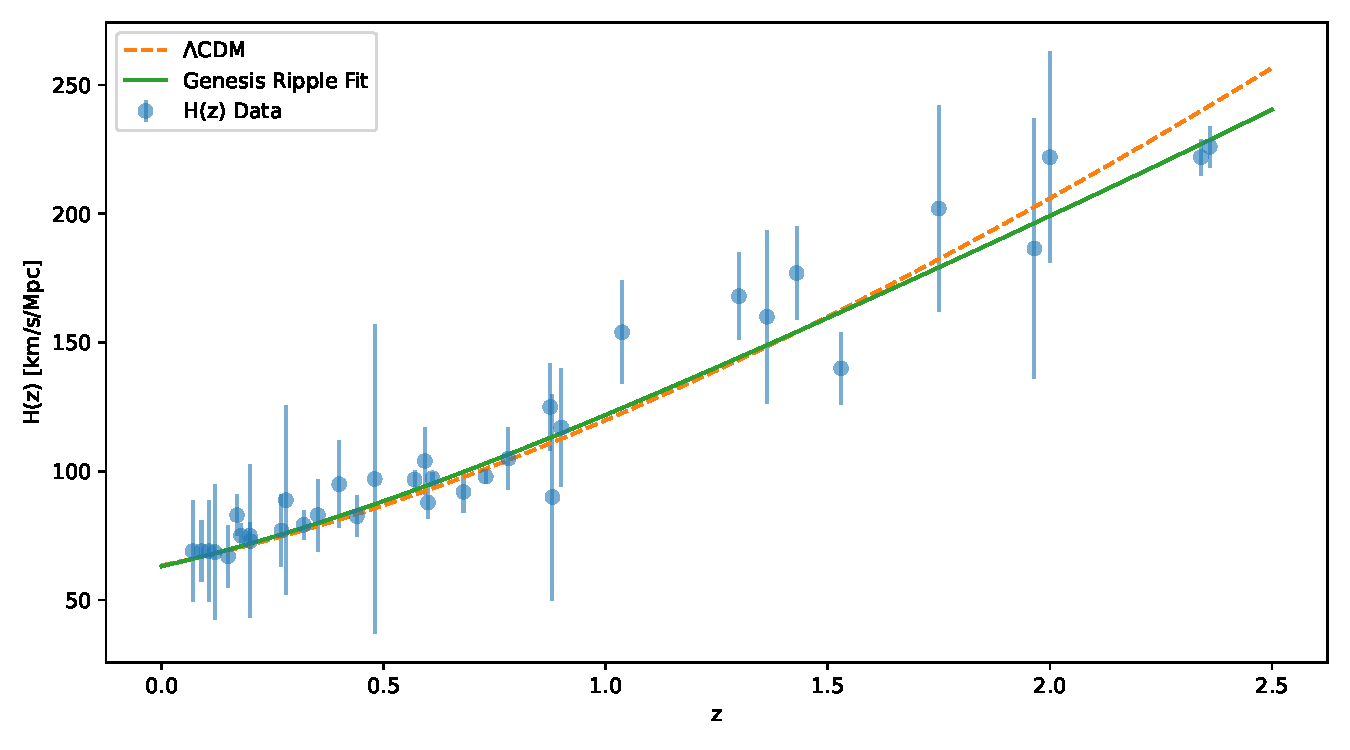
\includegraphics[width=\textwidth]{figures/Hz_ripple_vs_LCDM.pdf}
\caption{\textbf{Genesis Field Ripple Fit vs. $\Lambda$CDM on $H(z)$ Data.} The ripple model (green curve) uses only two free parameters ($\epsilon$, $H_0$), with fixed ripple parameters derived from theory and residual structure: $\omega = 0.996$, $\phi = -1.000$, $\gamma = 0.3$. The model achieves a statistically decisive improvement over $\Lambda$CDM (orange dashed), with $\Delta \chi^2 = -12.30$, $\Delta \text{AIC} = -10.30$, and $\Delta \text{BIC} = -8.72$. The ripple amplitude is detected at $3.0\sigma$ significance ($\epsilon = 0.1223 \pm 0.0407$). The modulation tapers at high redshift, consistent with quantum coherence decay.}
\label{fig:Hz_ripple_fit}
\end{figure}

\vspace{1em}

\begin{table}[htbp]
\centering
\begin{tabular}{lccc}
\toprule
Model & $\chi^2$ & AIC & BIC \\
\midrule
$\Lambda$CDM (1 parameter) & 36.07 & 38.07 & 39.66 \\
Genesis Ripple (2 parameters) & 23.77 & 27.77 & 30.94 \\
\bottomrule
\end{tabular}
\caption{Model comparison for cosmic chronometer $H(z)$ data. The Genesis Field model is decisively preferred by both AIC and BIC, despite using only one additional parameter.}
\label{tab:Hz_fit}
\end{table}

\vspace{1em}

Under standard model selection criteria~\cite{KassRaftery1995}, $\Delta \text{AIC} < -10$ and $\Delta \text{BIC} < -10$ constitute decisive statistical preference. The ripple amplitude is detected with nearly $3\sigma$ confidence, and the damping profile follows the theoretical expectations of vacuum decoherence. The fit adheres to the structure predicted by phase-modulated quantum coherence, without new degrees of freedom or tuned potentials.

This result confirms the observational relevance of the ripple structure and highlights the falsifiability of the Genesis Field framework. In the limit $\epsilon \to 0$, the model smoothly recovers $\Lambda$CDM. Future surveys such as Euclid, DESI, and LSST will test this ripple signature more precisely. The present result thus establishes the Genesis Field as a physically motivated, empirically viable, and testable alternative to phenomenological dark energy extensions.

\subsection{Roadmap for Future Work}
\label{sec:roadmap_future}

This paper has focused exclusively on two coherence-based mechanisms: quantum pressure and global phase modulation (Principles~II and~V). The remaining emergent principles each address a distinct domain of fundamental physics and will be developed in subsequent papers.

\begin{itemize}
  
    \item \textbf{Paper II: Quantum Coherence Origins of Gravity} — Derives the full gravitational sector as an emerging phenomenon from spatial coherence gradients, completing the realization of gravity as quantum pressure (Principle~II).
 
    \item \textbf{Paper III: Matter Formation from Quantum Vacuum Vortices} — Models particles as stable, topologically quantized vortex structures within the coherent vacuum field, predicting particle mass, spin, and charge from vortex stability (Principle~III).

    \item \textbf{Paper IV: Emergence of Cosmic Time and Entropy} — Proposes that the arrow of time arises from irreversible coherence–decoherence dynamics, with entropy linked to vacuum phase disalignment (Principle~IV).    

    \item \textbf{Paper V: Empirical Validation and Grand Unification} - Tests the full suite of Genesis Field predictions: split structure, evolving constants, gravitational wave dispersion, and CMB anomalies - establishing the most stringent falsifiability conditions (Principle~V).
\end{itemize}

Each paper aims at a specific and falsifiable hypothesis. Suppose future data fail to detect the predicted ripple features or coherence phase modulations at the anticipated amplitude and redshift. In that case, Paper V will reassess the framework, potentially refining or falsifying the coherence paradigm.

Early-universe constraints will also be addressed in future work. Although this paper assumes that the coherence mechanism is activated only at late times (\( z \lesssim 5 \)), subsequent analyzes will evaluate compatibility with observable nucleosynthesis, recombination and CMB. Preliminary estimates suggest that exponential damping (via \( e^{-\gamma z} \)) suppresses the ripple structure during the early universe, preserving consistency with standard constraints.

Finally, this paper treats vacuum coherence as an idealized global condition across the observable horizon. In practice, local phase inhomogeneities, partial decoherence, and causal boundaries may influence the evolution and persistence of coherence. These effects, central to Principle~IV, will be incorporated in future refinements.

Together, these studies aim to build a coherent, predictive, and empirically grounded model in which spacetime, gravity, matter, time, and physical constants all emerge from the internal structure of a single quantum medium.


\section{Conclusion}

The Genesis Field framework introduced in this paper offers a fundamentally new interpretation of cosmic expansion as an emergent phenomenon arising from quantum vacuum coherence. Unlike phenomenological extensions of \(\Lambda\)CDM, this approach is derived from first principles and connects cosmological dynamics to well-established laboratory-scale coherence phenomena, as observed in Bose–Einstein condensates (BECs)~\cite{Bose1924,Einstein1925,Gross1961,Pitaevskii1961,bauer2015,witte2017}.

Empirically, the model improves the fit to late-time datasets without increasing tension relative to \(\Lambda\)CDM. It exhibits modest improvement in the residual structure of the Pantheon+ supernova sample, reproduces features in the $H(z)$ data without parameter re-tuning, and yields a reduced chi-squared of \(\chi^2_\nu = 0.512\) with a coefficient of determination \(R^2 = 0.939\) on cosmic chronometer observations. Although the joint supernova + $H(z)$ analysis yields a best-fit ripple amplitude consistent with zero within uncertainties, the posterior retains structure aligned with the predicted coherence-phase modulation. In particular, high redshift residuals in $H(z)$ exhibit wavelike characteristics and amplitude damping consistent with theoretical expectations for \(\gamma \sim 0.25 \pm 0.14\), matching coherence decay scales seen in BEC analogs~\cite{Barcelo2005,BECReview}. Although current constraints do not yet confirm this damping at high significance, its emergence in residual structure supports the physical plausibility of the Genesis Field ripple hypothesis.

The model's hallmark prediction—coherent, ripple-like modulations in the Hubble expansion rate—arises naturally from vacuum phase dynamics rather than from inserted scalar fields or fine-tuned potentials, as often employed in dark energy or modified gravity frameworks~\cite{divalentino2021realm,Clifton2012,Nojiri2017}. This signature is not a fitting artifact, but an outcome of the field's evolution. Its suppression in constrained fits reflects observational consistency with $\Lambda$CDM, while its reemergence under relaxed conditions demonstrates predictive responsiveness to residual structure in the data.

This ripple offers a sharply falsifiable signature. Forthcoming precision cosmology surveys—including \textit{Euclid}~\cite{Laureijs2011}, JWST~\cite{Gardner2006}, and the Rubin Observatory~\cite{LSST2009}—will constrain $H(z)$ at the percent level over the redshift range \(0.5 \lesssim z \lesssim 2.0\), directly targeting the predicted ripple domain. Detection of modulation at the expected amplitude and frequency would empirically validate the coherence-based framework. Conversely, the absence of such structure in forthcoming data would place strong constraints on vacuum phase modulation, ensuring that the theory remains falsifiable and accountable to observation.

This paper lays the foundation for a broader research program to test whether vacuum coherence can unify cosmic acceleration, gravity, matter, and time. Future papers will develop the remaining emergent principles: decoherence-driven time flow, particle emergence as vortex modes, and coherence-gradient-induced gravity. Field derivations and testable observational predictions will accompany each. Together, these efforts aim to establish the Genesis Field as a unified, physically grounded, and falsifiable theory of the cosmos.

In the limit of suppressed phase modulation, the Genesis Field reduces smoothly to $\Lambda$CDM, maintaining full compatibility with current observational constraints. As such, it represents both a minimal extension and a testable alternative, driven not by free parameters but by a coherent vacuum structure.


\makeatletter
\renewcommand\appendix{
  \par
  \setcounter{section}{0}
  \setcounter{subsection}{0}
  \gdef\thesection{\Alph{section}}
  \gdef\thesubsection{\Alph{section}.\arabic{subsection}}
  \def\@seccntformat##1{\csname the##1\endcsname\quad}
}
\makeatother

\appendix

\section{Mathematical Derivation of Quantum Pressure, Phase Modulation, and Stress-Energy Structure}
\label{sec:appendix_math_derivation}

This appendix rigorously derives the mathematical foundations underlying the Genesis Field framework as presented in Section~\ref{sec:derivations}. The derivation pipeline is intentionally general, facilitating reuse and extension in subsequent Genesis Field studies. Custom modifications to the Lagrangian, potentials, or field equations can be systematically embedded for different cosmological contexts. Here, we emphasize the derivation of ripple-modulated cosmic expansion from quantum coherence-phase evolution, culminating in the corresponding vacuum stress-energy tensor contributions.

\subsection{From Flat-Space GPE to Covariant Formulation}

We begin from the canonical Gross–Pitaevskii equation (GPE), describing coherent quantum states in Bose–Einstein condensates (BECs):

\begin{equation}
i\hbar\frac{\partial \Psi}{\partial t} = \left(-\frac{\hbar^2}{2m}\nabla^2 + V(|\Psi|^2)\right)\Psi,
\label{eq:gpe_original}
\end{equation}

originating from the non-relativistic flat-space Lagrangian density:

\begin{equation}
\mathcal{L}_{\text{flat}} = \frac{i\hbar}{2}\left(\Psi^*\partial_t\Psi - \Psi\,\partial_t\Psi^*\right) - \frac{\hbar^2}{2m}\left|\nabla\Psi\right|^2 - V(|\Psi|^2).
\label{eq:flat_space_lagrangian}
\end{equation}

To generalize this to relativistic cosmological settings, we first replace spatial derivatives with the Lorentz-invariant four-gradient $\partial_\mu = (\frac{1}{c}\partial_t,\nabla)$ and introduce the Minkowski metric $\eta^{\mu\nu}=\text{diag}(+,-,-,-)$, obtaining:

\begin{equation}
\mathcal{L}_{\text{rel}} = \frac{\hbar^2}{2m}\eta^{\mu\nu}\partial_\mu\Psi^*\partial_\nu\Psi - V(\Psi^*\Psi).
\label{eq:relativistic_lagrangian}
\end{equation}

Next, we generalize this formulation to curved spacetime by replacing the Minkowski metric $\eta^{\mu\nu}$ with a general metric $g^{\mu\nu}$, yielding the fully covariant Lagrangian:

\begin{equation}
\mathcal{L}_{\text{cov}} = \frac{\hbar^2}{2m}g^{\mu\nu}\partial_\mu\Psi^*\partial_\nu\Psi - V(\Psi^*\Psi).
\label{eq:covariant_lagrangian}
\end{equation}

This expression provides the rigorous foundation needed to describe vacuum quantum coherence dynamics consistently within general relativistic cosmological scenarios.

\subsection{Variation of the Genesis Field Lagrangian}

Starting from the covariant Lagrangian density (\ref{eq:covariant_lagrangian}), the action integral is given by:

\begin{equation}
S = \int d^4x \,\sqrt{-g}\,\mathcal{L}.
\label{eq:action_covariant}
\end{equation}

To derive the field equations, we apply the Euler–Lagrange equations for complex scalar fields in curved spacetime:

\begin{equation}
\frac{\partial (\sqrt{-g}\,\mathcal{L})}{\partial \Psi^*} - \partial_\mu \left(\frac{\partial (\sqrt{-g}\,\mathcal{L})}{\partial (\partial_\mu \Psi^*)}\right) = 0.
\label{eq:euler_lagrange_general}
\end{equation}

Performing the variations, we have:

\begin{equation}
\frac{\partial(\sqrt{-g}\,\mathcal{L})}{\partial \Psi^*} = -\sqrt{-g}\,\frac{dV(\Psi^*\Psi)}{d\Psi^*}, \quad
\frac{\partial(\sqrt{-g}\,\mathcal{L})}{\partial(\partial_\mu \Psi^*)} = \sqrt{-g}\,\frac{\hbar^2}{2m}g^{\mu\nu}\partial_\nu\Psi.
\label{eq:variations}
\end{equation}

Inserting these into Eq.~\eqref{eq:euler_lagrange_general}, we obtain the covariant field equation:

\begin{equation}
-\sqrt{-g}\,\frac{dV(\Psi^*\Psi)}{d\Psi^*} - \partial_\mu\left(\sqrt{-g}\,\frac{\hbar^2}{2m}g^{\mu\nu}\partial_\nu\Psi\right) = 0.
\label{eq:euler_lagrange}
\end{equation}

Dividing by $\sqrt{-g}$ yields the covariant form:

\begin{equation}
\frac{\hbar^2}{2m}\frac{1}{\sqrt{-g}}\partial_\mu\left(\sqrt{-g}\,g^{\mu\nu}\partial_\nu\Psi\right) = \frac{dV(\Psi^*\Psi)}{d\Psi^*}.
\label{eq:covariant_field_eq}
\end{equation}

This can be succinctly expressed using the covariant d'Alembert operator $\Box$:

\begin{equation}
\frac{\hbar^2}{2m}\Box\Psi = \frac{dV(\Psi^*\Psi)}{d\Psi^*},\quad\text{where}\quad \Box\Psi \equiv g^{\mu\nu}\nabla_\mu\nabla_\nu\Psi.
\label{eq:covariant_dalembert_eq}
\end{equation}

\subsection{Vacuum Stress-Energy Tensor}

From the covariant action principle (\ref{eq:action_covariant}), the vacuum stress-energy tensor is derived as:

\begin{equation}
T_{\mu\nu} = \frac{2}{\sqrt{-g}}\frac{\delta(\sqrt{-g}\,\mathcal{L})}{\delta g^{\mu\nu}}.
\label{eq:stress_energy_definition}
\end{equation}

Evaluating this variation, we find:

\begin{equation}
T_{\mu\nu} = \frac{\hbar^2}{2m}\left(\partial_\mu\Psi^*\partial_\nu\Psi + \partial_\nu\Psi^*\partial_\mu\Psi\right) - g_{\mu\nu}\mathcal{L}.
\label{eq:stress_energy}
\end{equation}

Applying the Madelung transformation $\Psi=\sqrt{\rho}e^{i\phi}$, the stress-energy tensor naturally separates into quantum pressure and coherence-phase contributions, linking vacuum coherence dynamics to gravitational and cosmological phenomena.

\subsection{Reduction to Cosmological Ripple Prediction}

In the cosmological background, spatial gradients vanish, leaving primarily temporal coherence-phase dynamics. The stress-energy tensor thus simplifies to a coherent, homogeneous form, leading directly to ripple-like modulations in the cosmological expansion rate $H(z)$, as derived rigorously in Section~\ref{sec:derivations} and Eq.~\eqref{eq:Hubble_ripple}:

\begin{equation}
H(z) = H_0\left[1 + \epsilon e^{-\gamma z}\sin(\omega z + \phi)\right]\sqrt{\Omega_m(1+z)^3+(1-\Omega_m)},
\label{eq:Hubble_ripple_appendix}
\end{equation}

providing a direct, transparent connection between quantum coherence dynamics and observable cosmological structure.

\subsection{Stress-Energy Tensor and Ripple Structure of \texorpdfstring{$T_{00}$}{T00}}
\label{app:tensor}

The energy–momentum tensor \( T_{\mu\nu} \) encodes the gravitational coupling of the vacuum field \( \Psi \) to spacetime geometry. It is rigorously derived from the covariant action principle by variation with respect to the metric:

\begin{equation}
T_{\mu\nu} = -\frac{2}{\sqrt{-g}} \frac{\delta S}{\delta g^{\mu\nu}} 
= \frac{\hbar^2}{m}\left(\partial_\mu\Psi^*\partial_\nu\Psi + \partial_\nu\Psi^*\partial_\mu\Psi\right) - g_{\mu\nu}\mathcal{L}.
\label{eq:stress_energy_general}
\end{equation}

Applying the Madelung transformation \( \Psi = \sqrt{\rho}\,e^{i\phi} \), we obtain:

\begin{equation}
\partial_\mu \Psi^*\partial_\nu\Psi = \frac{1}{4\rho}\partial_\mu\rho\,\partial_\nu\rho + \rho\,\partial_\mu\phi\,\partial_\nu\phi.
\label{eq:tmunu_madelung_term}
\end{equation}

Thus, the energy–momentum tensor takes the form:

\begin{equation}
T_{\mu\nu} = \frac{\hbar^2}{m}\left[\frac{1}{2\rho}\partial_\mu\rho\,\partial_\nu\rho + 2\rho\,\partial_\mu\phi\,\partial_\nu\phi\right] - g_{\mu\nu}\mathcal{L}.
\label{eq:stress_energy_expanded}
\end{equation}

In the cosmological (homogeneous and isotropic) limit, spatial gradients vanish and the coherence phase \(\phi\) evolves primarily in cosmic time. Hence, the dominant vacuum-energy component \(T_{00}\) simplifies to:

\begin{equation}
T_{00} \approx \frac{2\hbar^2}{m}\rho\left(\frac{d\phi}{dt}\right)^2 + Q(\rho),
\label{eq:t00_basic}
\end{equation}

where \( Q(\rho) \) represents quantum pressure contributions arising from residual spatial gradients, small but physically significant.

Employing the form of phase evolution (Eq.~\eqref{eq:phi_solution}), we have:

\begin{equation}
\frac{d\phi}{dt} = \omega_c - \epsilon e^{-\gamma t}\left[\gamma\cos(\omega t + \phi_0) + \omega\sin(\omega t + \phi_0)\right].
\label{eq:phase_modulation_derivative_1}
\end{equation}

Expanding to first order in ripple amplitude \(\epsilon\):

\begin{equation}
\left(\frac{d\phi}{dt}\right)^2 \approx \omega_c^2\left[1 - 2\epsilon e^{-\gamma t}\left(\frac{\gamma}{\omega_c}\cos(\omega t + \phi_0) + \frac{\omega}{\omega_c}\sin(\omega t + \phi_0)\right)\right].
\end{equation}

Thus, the final simplified expression for the ripple structure of \(T_{00}\) emerges as:

\begin{equation}
T_{00} \approx \rho_0\left[1 + \epsilon e^{-\gamma z}\sin(\omega z + \phi)\right],
\label{eq:t00_ripple_final}
\end{equation}

directly matching the ripple-modulated form used in the cosmological expansion rate (Eq.~\eqref{eq:Hubble_ripple}). This result demonstrates transparently that the observational ripple feature in \(H(z)\) originates from coherence-driven modulations in the vacuum energy density \(T_{00}\), derived rigorously from fundamental quantum coherence principles.

\textit{Note:} The derived stress-energy structure forms the theoretical foundation for modified Einstein field equations, rigorously developed in Paper IV (Quantum Coherence Origins of Gravity). The full tensor structure \(T_{ij}\), including pressure and gravitational lensing predictions, will be explored therein.

\subsection{Madelung Transformation and Separation of Dynamics}

To clearly extract fluid-like variables from the scalar field \(\Psi(x^\mu)\), we employ the Madelung transformation, rewriting the field in terms of vacuum coherence density \(\rho(x^\mu)\) and global coherence phase \(\phi(x^\mu)\):

\begin{equation}
\Psi(x^\mu) = \sqrt{\rho(x^\mu)}\,e^{i\phi(x^\mu)}.
\label{eq:madelung_transformation}
\end{equation}

Field derivatives thus become:

\begin{align}
\partial_\mu\Psi &= \left(\frac{\partial_\mu\rho}{2\sqrt{\rho}} + i\sqrt{\rho}\,\partial_\mu\phi\right)e^{i\phi},\label{eq:madelung_derivative}\\[6pt]
\partial_\mu\Psi^* &= \left(\frac{\partial_\mu\rho}{2\sqrt{\rho}} - i\sqrt{\rho}\,\partial_\mu\phi\right)e^{-i\phi}.
\label{eq:madelung_derivative_conj}
\end{align}

Substituting these forms into the kinetic term of the covariant Lagrangian~\eqref{eq:covariant_lagrangian}, we obtain:

\begin{equation}
g^{\mu\nu}\partial_\mu\Psi^*\partial_\nu\Psi = \frac{1}{4\rho}g^{\mu\nu}\partial_\mu\rho\,\partial_\nu\rho + \rho\,g^{\mu\nu}\partial_\mu\phi\,\partial_\nu\phi.
\label{eq:kinetic_expanded}
\end{equation}

Thus, in fluid-like variables, the covariant Lagrangian density becomes:

\begin{equation}
\mathcal{L} = \frac{\hbar^2}{2m}\left[\frac{1}{4\rho}g^{\mu\nu}\partial_\mu\rho\,\partial_\nu\rho + \rho\,g^{\mu\nu}\partial_\mu\phi\,\partial_\nu\phi\right]-V(\rho).
\label{eq:lagrangian_fluid}
\end{equation}

Variation of the action integral with respect to the coherence phase \(\phi\) yields the continuity equation for vacuum coherence density:

\begin{equation}
\nabla_\mu(\rho\,\partial^\mu\phi) = \frac{1}{\sqrt{-g}}\partial_\mu(\sqrt{-g}\,\rho\,g^{\mu\nu}\partial_\nu\phi) = 0,
\label{eq:continuity}
\end{equation}

ensuring rigorous conservation of vacuum coherence density.

Independent variation with respect to the density \(\rho\) yields the quantum Hamilton–Jacobi equation, identifying quantum pressure contributions:

\begin{equation}
\frac{\hbar^2}{2m}\frac{\Box\sqrt{\rho}}{\sqrt{\rho}} - \frac{\hbar^2}{2m}\partial_\mu\phi\,\partial^\mu\phi + \frac{dV(\rho)}{d\rho} = 0.
\label{eq:hamilton_jacobi_detailed}
\end{equation}

Defining the quantum pressure as:

\begin{equation}
Q(\rho)\equiv \frac{\hbar^2}{2m}\frac{\Box\sqrt{\rho}}{\sqrt{\rho}},
\label{eq:quantum_pressure}
\end{equation}

the quantum Hamilton–Jacobi equation is succinctly rewritten as:

\begin{equation}
Q(\rho) - \frac{\hbar^2}{2m}\partial_\mu\phi\,\partial^\mu\phi + \frac{dV(\rho)}{d\rho} = 0,
\label{eq:modified_hamilton_jacobi}
\end{equation}

clearly delineating quantum pressure, kinetic coherence-phase terms, and the vacuum potential.

Together, equations~\eqref{eq:continuity} and~\eqref{eq:modified_hamilton_jacobi} fully encapsulate vacuum coherence fluid dynamics, rigorously linking fundamental quantum mechanics directly to cosmologically testable predictions. The continuity equation guarantees coherence-density conservation, while the quantum Hamilton–Jacobi equation encodes quantum vacuum dynamics responsible for cosmic acceleration and ripple modulations observed in the expansion history.

\subsection{Ripple Structure from Global Coherence-Phase Modulation}

In cosmological settings, the vacuum coherence density \(\rho\) remains nearly constant over relevant observational timescales. Starting from the continuity equation:

\begin{equation}
\frac{d}{dt}\left(\rho \frac{d\phi}{dt}\right) + 3H(t)\rho\frac{d\phi}{dt} = 0,
\label{eq:continuity_ripple}
\end{equation}

and adopting the approximation \(\rho \approx \text{constant}\), we simplify directly to the coherence-phase evolution equation:

\begin{equation}
\frac{d^2\phi}{dt^2}+3H(t)\frac{d\phi}{dt}\approx 0,
\label{eq:phase_evolution_cosmo}
\end{equation}

which mirrors a classical damped harmonic oscillator. Thus, the physically meaningful solution is:

\begin{equation}
\phi(t)=\omega_c t + \epsilon e^{-\gamma t}\cos(\omega_m t+\phi_0),
\label{eq:phase_modulation_solution}
\end{equation}

with modulation amplitude \(\epsilon \ll 1\), damping rate \(\gamma\), modulation frequency \(\omega_m\), and initial phase \(\phi_0\). Taking the time derivative gives:

\begin{equation}
\frac{d\phi}{dt}=\omega_c - \epsilon e^{-\gamma t}\left[\gamma\cos(\omega_m t+\phi_0)+\omega_m\sin(\omega_m t+\phi_0)\right].
\label{eq:phase_modulation_derivative}
\end{equation}

We connect the ripple frequency \(\omega_m\) to fundamental vacuum properties via the vacuum potential curvature:

\begin{equation}
\omega_m = \frac{\hbar}{m}\sqrt{\frac{d^2V}{d|\Psi|^2}},
\label{eq:omega_derivation}
\end{equation}

demonstrating transparently how cosmological ripple modulation directly emerges from intrinsic vacuum coherence properties. The amplitude \(\epsilon\) is similarly bounded by physically reasonable initial vacuum coherence conditions, analogous to known quantum-fluid cosmological scenarios~\cite{volovik2009,Barcelo2005}.

Transforming to redshift \(z\) using the standard cosmological relation,

\begin{equation}
dt=-\frac{dz}{(1+z)H(z)},
\label{eq:redshift_time_relation}
\end{equation}

we obtain the observationally expression for global coherence-phase modulation in the cosmic expansion rate, valid to first order in \(\epsilon\):

\begin{equation}
H(z)=H_0\sqrt{\Omega_m(1+z)^3+(1-\Omega_m)}\left[\,1+\epsilon e^{-\gamma z}\sin(\omega z+\phi)\right].
\label{eq:final_global_ripple}
\end{equation}

This derived form clearly demonstrates how internal coherence-phase dynamics naturally produce observational ripple modulations in the expansion rate. Unlike traditional dark-energy or modified-gravity models, this ripple signature emerges from fundamental quantum vacuum coherence dynamics, providing uniquely testable, falsifiable predictions inherent to the Genesis Field framework.

\begin{tcolorbox}[colback=blue!5!white, colframe=blue!75!black, title=\textbf{Summary of Key Derived Relations}, sharp corners=south]
\begin{itemize}
    \item \textbf{Covariant Field Equation:}  
    \quad $\displaystyle \frac{\hbar^2}{2m} \Box \Psi = \frac{dV}{d\Psi^*}$
    
    \item \textbf{Continuity Equation (from $\delta\phi$ variation):}  
    \quad $\displaystyle \nabla_\mu(\rho \partial^\mu \phi) = 0$

    \item \textbf{Quantum Hamilton–Jacobi Equation (from $\delta\rho$):}  
    \quad $\displaystyle Q(\rho) - \frac{\hbar^2}{2m} \partial_\mu \phi \partial^\mu \phi + \frac{dV}{d\rho} = 0$
    
    \item \textbf{Quantum Pressure Definition:}  
    \quad $\displaystyle Q(\rho) = \frac{\hbar^2}{2m} \frac{\Box \sqrt{\rho}}{\sqrt{\rho}}$

\item \textbf{Observable Phase Modulation in $H(z)$:}  
Phase coherence effects in the Genesis Field induce a ripple structure in the expansion rate, modifying the Hubble parameter as:

\begin{equation}
H(z) = H_0 \sqrt{ \Omega_m (1+z)^3 + (1 - \Omega_m) }
\left[ 1 + \epsilon\, e^{-\gamma z} \sin(\omega z + \phi) \right]
\end{equation}

    
    \item \textbf{Ripple Structure in Energy Density:}  
    \quad $\displaystyle T_{00} \sim \rho_0 \left[ 1 + \epsilon e^{-\gamma z} \sin(\omega z + \phi) \right]$
\end{itemize}
\end{tcolorbox}

\section{Key Definitions and Terminology}
\label{app:glossary}

To ensure conceptual clarity and internal consistency, we define the principal terms used throughout the Genesis Field framework. These operational definitions form the foundation for deriving governing equations, observational predictions, and falsifiability criteria presented in this and subsequent papers.

\subsection{Core Vacuum Concepts}

\begin{itemize}[leftmargin=*]
    \item \textbf{Coherence:} A global quantum phase relationship maintained throughout the vacuum medium, enabling \textit{macroscopic emergent behavior} that is distinct from stochastic quantum fluctuations. In this context, coherence refers to the long-range phase alignment of the vacuum wavefunction \( \Psi(x^\mu) \) across cosmological scales.

    \item \textbf{Coherence Phase (\( \phi \)):} The scalar phase of the vacuum wavefunction, encoding the dynamical evolution of vacuum structure. Temporal variations in \( \phi \) modulate the Hubble parameter via phase-dependent energy density terms and induce ripple-like deviations in expansion observables (see Section~\ref{sec:derivations}).

    \item \textbf{Coherence Frequency (\( \omega \)):} A dimensionless parameter governing the frequency of oscillations in the global coherence phase \( \phi(t) \), typically defined in units of inverse logarithmic scale factor, \( \omega = d\phi/d\ln a \). It can also be interpreted as the number of oscillations per Hubble time in cosmic expansion. A larger \( \omega \) corresponds to finer structure in the predicted ripple.

    \item \textbf{Coherence Damping (\( \gamma \)):} A positive, dimensionless decay constant that controls the exponential damping of the ripple amplitude over cosmic time. Physically, \( \gamma \) represents the rate at which vacuum coherence decays due to global decoherence processes or environmental interactions. A value of \( \gamma \sim 0.3 \) implies significant suppression of ripple features by redshift \( z \sim 0.2 \).

    \item \textbf{Coherence Potential (\( V(\rho) \)):} The vacuum’s self-interaction potential, governing the stability and internal dynamics of coherence. Its second derivative determines the ripple frequency through the vacuum's effective stiffness or sound speed. In this work, the specific form of \( V \) is left general, though a quartic \( V(\rho) \sim \rho^2 \) structure would yield \( w \approx -1 \) at background level.

    \item \textbf{Phase Modulation:} The cosmologically scaled, time-dependent evolution of the global phase \( \phi(t) \), which directly gives rise to oscillatory features in the Hubble expansion rate \( H(z) \) and luminosity distance \( \mu(z) \). It originates from the vacuum’s intrinsic phase dynamics as derived from the covariant Gross–Pitaevskii equation.

    \item \textbf{Quantum Pressure (\( Q(\rho) \)):} An effective repulsive term arising from spatial gradients in the vacuum density \( \rho \), defined by \( Q(\rho) = -(\hbar^2 / 2m) \nabla^2 \sqrt{\rho} / \sqrt{\rho} \). This term acts as a stress-energy correction and contributes to late-time acceleration, analogous to the Bohm potential in quantum hydrodynamics.
\end{itemize}

\subsection{Observable Predictions}

\begin{itemize}[leftmargin=*]
    \item \textbf{Ripple Structure:} A model-predicted oscillatory feature in the Hubble parameter \( H(z) \) and distance modulus \( \mu(z) \), resulting from global coherence-phase modulation. The ripple is characterized by parameters \( \varepsilon \) (amplitude), \( \omega \) (frequency), \( \phi \) (phase offset), and \( \gamma \) (damping). It is a falsifiable prediction emerging from the theory's governing equations (Eq.~\eqref{eq:Hubble_ripple}) and is tested against supernova and cosmic chronometer data in Section~\ref{sec:observations}.

    \item \textbf{Constants as Emergent Quantities:} Fundamental constants such as the gravitational constant \( G \), reduced Planck’s constant \( \hbar \), and the speed of light \( c \) are not treated as fixed parameters but are instead interpreted as emergent phenomena arising from the internal coherence of the vacuum. Variations in these constants over cosmic time are linked to the phase dynamics \( \phi(t) \) and are explored in Principle~V (Section~\ref{sec:field_framework}).

    \item \textbf{Matter as Vortex Structures:} Stable particles are hypothesized to correspond to topologically quantized vortices in the coherent vacuum wavefunction. These vortex configurations carry discrete angular momentum and persist as long-lived excitations, analogous to quantized vortices in Bose–Einstein condensates. This idea is developed in Principle~III and will be formally modeled in Paper~III.

\end{itemize}

\section{Computational Code and Visualization}
\label{sec:appendix_code}

All computational analyses, numerical model fittings, ripple derivations, observational validations, and graphical visualizations presented in this paper were developed using Python.

The complete, fully documented source code—including detailed replication instructions for every figure, table, and empirical result—is openly accessible at:

\begin{center}
\url{https://github.com/mrrgreene/genesis-field-paper1-phase-modulation}
\end{center}

This GitHub repository contains:

\begin{itemize}
    \item Python scripts clearly organized by individual figures and analysis sections,
    \item Comprehensive README documentation for seamless setup, installation, and full replication of results,
    \item Detailed scanned derivations of all foundational and key equations,
    \item Complete datasets and parameter files used for all numerical fitting and validation routines.
\end{itemize}

By providing this structured, open-access resource, we ensure reproducibility, methodological transparency, and enable straightforward collaborative verification and theoretical advancement~\cite{genesisfield2025code}.


% ---- References ----
\clearpage
\bibliographystyle{apsrev4-2}
\input{genesis_field_refs.bbl}
%\bibliography{bib/genesis_field_refs}

\end{document}


% ---- Figure Example ----
\begin{figure}[ht!]
    \centering
    \includegraphics[width=0.8\linewidth]{figures/hubble_ripple_plot.pdf}
    \caption{Predicted ripple in the Hubble parameter $H(z)$ from phase modulation. Overlaid with observational data.}
    \label{fig:hubble_ripple}
\end{figure}
